\documentclass[12pt,onecolumn,conference]{IEEEtran}

% ---------------------------------------------------------------------------
% Language and fonts
% ---------------------------------------------------------------------------
\usepackage[utf8]{inputenc}
\usepackage[T1]{fontenc}
\usepackage[english]{babel}

% ---------------------------------------------------------------------------
% Page geometry
% ---------------------------------------------------------------------------
\usepackage[margin=2.5cm]{geometry}

% ---------------------------------------------------------------------------
% Units and quantities
% ---------------------------------------------------------------------------
\usepackage{siunitx}
\sisetup{per-mode=symbol}
\DeclareSIUnit\byte{B}
\DeclareSIUnit\GHz{\giga\hertz}

% ---------------------------------------------------------------------------
% Graphics and figures
% ---------------------------------------------------------------------------
\usepackage{graphicx}
\graphicspath{{figures/}}
\usepackage{caption}
\usepackage{float}
\usepackage{booktabs}
\usepackage{array}
\usepackage{tabularx}
\renewcommand{\tabularxcolumn}[1]{m{#1}}

% ---------------------------------------------------------------------------
% Code listings
% ---------------------------------------------------------------------------
\usepackage[dvipsnames]{xcolor}
\usepackage{listings}
\lstdefinestyle{codestyle}{
    basicstyle=\ttfamily\small,
    keywordstyle=\color{blue},
    commentstyle=\color{OliveGreen},
    stringstyle=\color{purple},
    numbers=left,
    numberstyle=\tiny\color{gray},
    stepnumber=1,
    numbersep=8pt,
    backgroundcolor=\color{black!3},
    frame=single,
    breaklines=true,
    breakatwhitespace=false,
    showstringspaces=false,
    tabsize=4
}
\lstset{style=codestyle}

% ---------------------------------------------------------------------------
% Hyperlinks and cross-referencing
% ---------------------------------------------------------------------------
\usepackage[hidelinks]{hyperref}

% ---------------------------------------------------------------------------
% Page style: centered page numbers, running header
% ---------------------------------------------------------------------------
\usepackage{fancyhdr}
\pagestyle{fancy}
\fancyhf{}
\fancyhead[L]{Transition History for Single-BS CSI Localization}
\fancyhead[R]{Battat et al.}
\fancyfoot[C]{\thepage}
\renewcommand{\headrulewidth}{0.4pt}
\renewcommand{\footrulewidth}{0pt}

\fancypagestyle{titlepage}{
  \fancyhf{}
  \fancyfoot[C]{\thepage}
  \renewcommand{\headrulewidth}{0pt}
}

% ---------------------------------------------------------------------------
% Section heading styling
% ---------------------------------------------------------------------------
\usepackage{titlesec}
\titleformat{\subsection}
  {\normalfont\normalsize\bfseries\itshape}
  {\thesubsectiondis}
  {0.5em}
  {}
\titlespacing*{\subsection}{0pt}{1.5ex plus 1.5ex minus 0.5ex}{0.7ex plus .5ex minus 0ex}
\titleformat{\subsubsection}
  {\normalfont\normalsize\bfseries}
  {}
  {0pt}
  {}
\titlespacing*{\subsubsection}{0pt}{1.5ex plus 1.5ex minus 0.5ex}{0.7ex plus .5ex minus 0ex}

% ---------------------------------------------------------------------------
% Miscellaneous
% ---------------------------------------------------------------------------
\usepackage{enumitem}
\usepackage{amsmath}
\usepackage{amssymb}

% ---------------------------------------------------------------------------
% Review/annotation commands
% ---------------------------------------------------------------------------
\newcommand\asl[1]{{\bf\color{red}$<$ASL: #1$>$}}
\newcommand\uncertain[1]{{\color{orange}#1}}
% Content waiting for Gilad's diagnostic run and result push (Gilad Diagnostic 2026-10/).
% Remove every \pending{} before submission.
\newcommand\pending[1]{{\color{magenta}#1}}

% ---------------------------------------------------------------------------
% Title page metadata
% ---------------------------------------------------------------------------
% Title wording is the author's call; this is the working title.
\title{Transition History for Single-BS 5G NR CSI Localization:\\Model-Agnostic Gains and Their Hardware Dependence}
\author{
  \IEEEauthorblockN{Gilad Battat\IEEEauthorrefmark{1},
                    Alon S.~Levin\IEEEauthorrefmark{2},
                    David Sarne\IEEEauthorrefmark{1},
                    Sarit Kraus\IEEEauthorrefmark{1}}
  \IEEEauthorblockA{\IEEEauthorrefmark{1}Department of Computer Science, Bar-Ilan University}
  \IEEEauthorblockA{\IEEEauthorrefmark{2}Department of Electrical Engineering, Columbia University}
}
\date{Month Year}

\begin{document}

\maketitle
\thispagestyle{titlepage}

\begin{center}
\textit{Technical Report prepared for the IISAC Consortium}\\
\textit{Industry Partners: CEVA, Cellcom}
\end{center}

\newpage
\begin{abstract}
\pending{[Awaiting Gilad's results: the abstract is written once the mechanism experiment is in, since its outcome decides how the central claim is stated.]}
\end{abstract}


% \newpage \tableofcontents

\newpage
\section{Introduction}
\label{sec:introduction}

\subsection{Motivation}
\label{subsec:motivation}

% src: technical_documentation.md §1.1; FINAL_REPORT.md §1.1 (carried over from Project Report/1_introduction.tex)
Fifth- and sixth-generation cellular networks make several channel-derived measurements available natively at the base station~(BS): received signal strength~(RSS), signal-to-interference-plus-noise ratio~(SINR), angle of arrival~(AoA), and timing advance, none of which require dedicated positioning infrastructure to collect. %TODO-CITE: 3GPP Release 16 positioning-as-network-service framing
Turning these measurements into a position estimate for the user equipment~(UE) is motivated by applications ranging from emergency response and asset tracking to network-assisted navigation, and the need is sharpest precisely where satellite positioning is weakest: urban canyons, tunnels, and indoor spaces, where signal blockage and multipath substantially degrade the accuracy of the Global Positioning System~(GPS). %TODO-CITE: GNSS degradation in urban-canyon and indoor environments
Cellular positioning targets this gap directly, since a device already in radio contact with a BS can in principle be localized from measurements the network is collecting regardless of whether positioning was requested, with no added receiver and no sensor on the device itself.

% src: technical_documentation.md §1.1; FINAL_REPORT.md §1.1
The obstacle is accuracy rather than availability. RSS, the most universally reported of these metrics, is set primarily by distance from the BS, with multipath structure and shadow fading contributing only a secondary correction, which on its own leaves position under-constrained.

% src: FINAL_REPORT.md §2, "Geometric methods" paragraph
Multi-BS geometric positioning resolves the missing bearing directly, but only given multiple synchronized anchors or a high-quality angle estimate. %TODO-CITE: canonical ToA/TDoA/AoA multilateration reference(s)
A single serving BS has neither by default. That is what makes it the harder deployment case, and the more consequential one: it is exactly the setting in which a network already capable of collecting these measurements would most benefit from a fix that adds no new infrastructure.

\subsection{The Distance-Ring Ambiguity and the Hypothesis}
\label{subsec:ambiguity-hypothesis}

% src: FINAL_REPORT.md §1.1, §3.2
Let $\mathbf{p}_{UE}$ and $\mathbf{p}_{BS}$ denote the UE and serving-BS positions, and let $r = \lVert \mathbf{p}_{UE} - \mathbf{p}_{BS} \rVert$ be their range. Under a log-distance path-loss model,
\begin{equation}
  \mathrm{RSS} \approx P_{tx} - 10\gamma\log_{10} r + \chi,
  \label{eq:path-loss}
\end{equation}
with $\gamma$ the path-loss exponent and $\chi$ zero-mean shadow fading of standard deviation~$\sigma$. The map from RSS to position is therefore one-to-many: a static measurement identifies $r$, up to $\chi$, but leaves bearing entirely unconstrained. Locations on a common range ring around the BS are consequently indistinguishable to a static, single-snapshot estimator, which is the \emph{distance-ring ambiguity}. The ambiguity is worst in geometries dominated by line-of-sight~(LOS) propagation, where the range-to-RSS map is close to monotone and multipath diversity is minimal. SINR and AoA can each supply the missing bearing information, but both are conditional: SINR depends on interferer placement and calibration, and AoA depends on UE beamforming hardware that a large share of connected devices does not have.

% src: FINAL_REPORT.md §1.2
The hypothesis evaluated in this report is that a moving UE's measurement sequence encodes more positional information than any single snapshot, and that this holds regardless of the estimator applied on top of it. Two positions on the same range ring produce the same instantaneous RSS but different trajectories through measurement space, because the local channel neighborhood around each position is different and evolves differently as the UE moves.

% src: FINAL_REPORT.md §3.3 (window definition)
Formally, let $\mathbf{m}(t)$ denote the vector of channel-derived measurements reported for the UE at discrete snapshot time~$t$~(Table~\ref{tab:nomenclature}). Given a history depth~$h$, the model input is the window of $h+1$ consecutive observations,
\begin{equation}
  \mathcal{W}_h(t) = \left[\, \mathbf{m}(t-h),\ \dots,\ \mathbf{m}(t) \,\right],
  \label{eq:transition-history}
\end{equation}
where $h=0$ recovers the static, memoryless fingerprint as a special case. For $h>0$, $\mathcal{W}_h(t)$ makes the temporal derivatives of $\mathbf{m}$ observable; Section~\ref{sec:system-model} sets out what those derivatives can and cannot constrain.

% -------------------------------------------------------
% Nomenclature / notation table
% Extend this table as new symbols are introduced; keep symbol
% usage consistent with this list throughout the report.
% -------------------------------------------------------
\begin{table}[h]
  \centering
  \caption{Nomenclature}
  \label{tab:nomenclature}
  \begin{tabular}{@{}ll@{}}
    \toprule
    Symbol & Description \\
    \midrule
    $\mathbf{m}(t)$ & Measurement vector at snapshot time~$t$ \\
    $h$ & History depth~(number of prior snapshots in the window) \\
    $\mathcal{W}_h(t)$ & History window, $[\mathbf{m}(t-h),\dots,\mathbf{m}(t)]$ \\
    $\mathbf{p}_{UE}$, $\mathbf{p}_{BS}$ & UE and serving-BS positions \\
    $r$ & UE--BS range, $r = \lVert \mathbf{p}_{UE} - \mathbf{p}_{BS} \rVert$ \\
    $\theta_{az}$, $\theta_{el}$ & AoA azimuth and elevation \\
    $\gamma$ & Path-loss exponent \\
    $\chi$ & Zero-mean shadow-fading term, standard deviation $\sigma$ \\
    $\sigma_r$ & Range uncertainty implied by RSS alone \\
    $N_{ant}$ & UE antenna count \\
    $\Delta t$ & Time between consecutive snapshots of one UE \\
    \bottomrule
  \end{tabular}
\end{table}


% Contributions and Scope subsections: drafted in _draft_contributions_scope.tex, linked after author review.

\section{Related Work}
\label{sec:related-work}

% src: FINAL_REPORT.md §2, "Fingerprinting" paragraph
Classical RSS fingerprinting matches a measurement snapshot against a surveyed database~\cite{yang2013_rssitocsi}; single-site multipath fingerprinting establishes that one BS already observes enough structure to localize without triangulation~\cite{kupershtein2013}, the principle this work extends to a moving user. Fingerprinting's characteristic failure mode is poor discrimination between points at equal range from the BS, which is exactly the distance-ring ambiguity the transition-history mechanism targets~(Section~\ref{subsec:ambiguity-hypothesis}). The static, $h=0$ $k$-nearest-neighbor regressor used as a baseline throughout this report stands in for this family. % src: FINAL_REPORT.md §2 (k-NN h=0 baseline)

% src: FINAL_REPORT.md §2, "Geometric methods" paragraph
Geometric methods recover position from an explicit system built on time-of-arrival, time-difference-of-arrival, or AoA estimates.
%TODO-CITE: canonical ToA/TDoA/AoA multilateration reference(s)
These methods require either multiple synchronized BSs or a high-quality angle estimate, so the single-serving-BS, single-angle-source deployment studied here is precisely the regime in which the geometric system is underdetermined: for a device that reports no angle at all, the available geometry constrains range but leaves bearing unresolved.

% src: FINAL_REPORT.md §2, "Sequence models for CSI" paragraph
Recurrent and dynamic-system formulations have likewise been applied to channel state information~(CSI)-based tracking~\cite{fang2010dynamic,yu2020rnn,shi2018tracking}, and a related line shows that the temporal autocorrelation of RSS improves fingerprinting accuracy when the signal is treated as a stationary process observed at a fixed location~\cite{wang2016temporal,tian2018temporal}. That precursor is complementary rather than nested: its temporal signal is order-invariant and is aggregated across access points, so it survives for a stationary receiver and vanishes for a moving one, whereas the transition-history window used here is ordered, is read from a single BS, and encodes exactly the motion the in-place statistic discards. More broadly, this body of work motivates a new architecture and reports that it lowers error; the framing adopted here instead holds the estimator family fixed and varies only the input window, isolating the effect of the input transformation from the choice of architecture and allowing the comparison to extend by design to model families not tested in this report.

\section{System Model and Problem Formulation}
\label{sec:system-model}

\subsection{Measurement Model}
\label{subsec:measurement-model}

% src: FINAL_REPORT.md §3.1
At discrete snapshot time~$t$ the serving BS observes
\begin{equation}
  \mathbf{m}(t) = \big[\, \mathrm{RSS}(t),\ \mathrm{SINR}(t),\ \theta_{az}(t),\ \theta_{el}(t) \,\big],
  \label{eq:measurement-vector}
\end{equation}
with the azimuth/elevation pair $(\theta_{az}, \theta_{el})$ present only for UEs whose antenna count $N_{ant} \ge 2$. Multi-antenna UEs are modeled by maximum-ratio combining over the per-element channel,
\begin{equation}
  H_{\text{eff}}(f) = \sqrt{\textstyle\sum_{i=1}^{N_{ant}} \lvert H_i(f) \rvert^2},
  \label{eq:mrc}
\end{equation}
with a device-specific antenna-gain offset applied additively in dB. Throughout this report, UEs with $N_{ant} \ge 2$ are referred to as multi-antenna devices and UEs with $N_{ant} = 1$ as single-antenna devices.

\subsection{What History Can Add}
\label{subsec:history-dof}

% src: FINAL_REPORT.md §3.3
Over the window $\mathcal{W}_h(t)$ of Equation~(\ref{eq:transition-history}), an estimator can form finite differences of the measurements, of which two carry geometric meaning. The rate of change of RSS,
\begin{equation}
  \frac{d\,\mathrm{RSS}}{dt} \approx -\frac{10\gamma}{\ln 10} \cdot \frac{\dot r}{r},
  \label{eq:drss-dt}
\end{equation}
reflects the component of motion along the BS bearing, and the angular rate,
\begin{equation}
  \dot\theta_{az} = \frac{v_\perp}{r},
  \label{eq:dtheta-dt}
\end{equation}
where AoA is available, gives the tangential component of the velocity $v_\perp$ and, jointly with $\dot r$, the heading. For a UE moving at roughly constant speed, the pair $(\dot r, \dot\theta_{az})$ constrains position to the intersection of a range ring and a motion-consistent arc, a far smaller set than the ring alone.

% src: FINAL_REPORT.md §7.5 (dRSS/dr expression); Equation (path-loss) above
Without AoA, only the first of these is available, and its usefulness is bounded by the path-loss gradient. Differentiating Equation~(\ref{eq:path-loss}) with respect to range gives
\begin{equation}
  \left\lvert \frac{d\,\mathrm{RSS}}{dr} \right\rvert = \frac{10\gamma}{r \ln 10}\ \text{dB/m},
  \label{eq:rss-gradient}
\end{equation}
so a step of fixed length moves RSS by an amount that falls as $1/r$, while the shadow-fading term $\chi$ does not shrink with range. A sequence of RSS values can therefore carry useful information about motion relative to the BS only where the per-step change is not swamped by $\sigma$; how far from the BS that condition holds is an empirical question that the two study scales in this report bracket from either side.

\subsection{Task Formulations}
\label{subsec:task-formulations}

% src: FINAL_REPORT.md §3.4; technical_documentation.md §7.4 (625-class memory limit)
Two task formulations are evaluated. Classification predicts one of $G$ discrete grid cells, and is appropriate when grid spacing greatly exceeds position jitter. Regression predicts a continuous position relative to the serving BS and is scored by the 2D Euclidean error in meters. Regression is used for the larger deployment, where a $625$-class classifier proved memory-prohibitive and where evaluation is over unseen users rather than unseen time steps of known users.

\section{Experimental Setup}
\label{sec:setup}

\subsection{Channel Simulation}
\label{subsec:channel-simulation}

% src: FINAL_REPORT.md §4.2
All data is generated with a 3GPP TR~38.901-compliant channel simulator %TODO-CITE: QuaDRiGa channel simulator and 3GPP TR 38.901 channel model.
% src: configs (*_15x15, *_25x25: bandwidth 1e8); FINDINGS.md §2.1 (early single-user grid sweeps: 20 MHz, 3.5 GHz)
at $100\,\text{MHz}$ bandwidth~(the early single-user grid sweeps used $20\,\text{MHz}$), $256$ orthogonal frequency-division multiplexing~(OFDM) subcarriers, $30\,\text{dBm}$ transmit power per site, and an omnidirectional BS antenna element. The simulator's spatial-consistency model is the physical precondition for the mechanism under test: the channel evolves continuously along a UE's trajectory rather than being redrawn independently at each step, so consecutive snapshots carry correlated, motion-dependent structure. This work extends a time-aware multi-user massive multiple-input multiple-output~(MIMO) simulation infrastructure developed within the same research group, adding grid-constrained trajectory generation and the device-heterogeneity model of Section~\ref{subsec:device-model}. %TODO-CITE: upstream 5G Massive MIMO time-aware simulator (Israeli)

% src: FINAL_REPORT.md §4.2 ("What interference means here")
Where a deployment includes interfering BSs in addition to the serving BS, SINR is computed as
\begin{equation}
  \mathrm{SINR} = \frac{P_{\text{serving}}}{\sum_i P_{\text{IBS-}i} + P_{\text{noise}}}, \qquad P_{\text{noise}} = -104\,\text{dBm},
  \label{eq:sinr}
\end{equation}
so interference is contributed only by the modeled interfering sites. No user-to-user coupling is represented: users simulated in a shared batch share large-scale channel parameters, but a user's SINR does not depend on how many other users are simulated alongside it.

\subsection{Studies}
\label{subsec:studies}

% src: FINAL_REPORT.md §4.1, §7.5 ("eight differences"); technical_documentation.md §3, §7.1, §7.3.3, §7.4; configs/multi_user_voronoi_15x15_config.jsonc, ne_bs_voronoi_15x15_config.jsonc, ne_bs_voronoi_25x25_config.jsonc (center_frequency, grid, base_station)
The evidence comes from three simulated deployments at two scales, summarized in Table~\ref{tab:studies}. The \emph{controlled-grid study} places UEs on a $15\times15$ grid at $2\,\text{m}$ pitch within $20\,\text{m}$ of the serving BS and predicts the exact cell, under conditions chosen to be clean and repeatable; a single-user variant of the same set-up sweeps the grid from $3\times3$ to $20\times20$ cells. The \emph{macro-cell study} places $300$ users on a $25\times25$ grid at $4\,\text{m}$ pitch, $21$ to $157\,\text{m}$ from an off-grid serving BS, predicts continuous position, and evaluates on users never seen during training. The \emph{single-user $25\times25$ regression runs} share the macro-cell geometry but follow one user, split in time, and are used here only for the case of RSS and SINR without AoA. A fixed history depth of $h=3$ is used in the controlled-grid study and $h=5$ in the macro-cell study, with sweeps over $h$ where stated.

\begin{table}[h]
  \centering
  \caption{The three simulated deployments. The macro-cell study is reported per device group throughout.}
  \label{tab:studies}
  \small
  \begin{tabularx}{\textwidth}{@{}lXXX@{}}
    \toprule
     & Controlled-grid study & Single-user $25\times25$ runs & Macro-cell study \\
    \midrule
    Task & Classification~(225 cells) & Regression & Regression \\
    Grid, pitch & $15\times15$, $2\,\text{m}$ & $25\times25$, $4\,\text{m}$ & $25\times25$, $4\,\text{m}$ \\
    Service area & $28\times28\,\text{m}$ & $96\times96\,\text{m}$ & $96\times96\,\text{m}$ \\
    Range to serving BS & $0$--$20\,\text{m}$~(center BS); $21$--$61\,\text{m}$~(corner BS) & $21$--$157\,\text{m}$ & $21$--$157\,\text{m}$, mean $93\,\text{m}$ \\
    Carrier & $3.5\,\text{GHz}$ & $3.0\,\text{GHz}$ & $3.0\,\text{GHz}$ \\
    Population & 5 device profiles, $450{,}005$ samples & 1 user & 300 users simulated, 232 retained, 47 tested per split \\
    Split & Chronological $80/20$ within each user & Chronological, or shuffled 5-step blocks & $80/20$ over disjoint users \\
    Mobility & Random walk, $1.5\,\text{m/s}$ & Random walk & Four patterns, $0.1$--$15\,\text{m/s}$ \\
    AoA impairment & SINR-dependent noise, $5^\circ$ quantization & AoA not used in the runs cited & $4^\circ$ Gaussian noise, $5^\circ$ quantization \\
    Repetitions & Single run & Single run & Five seeds for headline comparisons \\
    \bottomrule
  \end{tabularx}
\end{table}
% src (macro-cell AoA impairment): CSI-Location src/python/utils/csi_dataset.py load_and_prepare_data (aoa_noise_std_deg=4.0, aoa_quant_step_deg=5.0); 232 retained: FINAL_REPORT.md §4.3; 47 test users: seed_repeats_all_models_summary.json per-run n_test_users; range 21.2-157.0 m, mean 93.2: FINAL_REPORT.md §7.5

% src: configs/multi_user_voronoi_15x15_config.jsonc (BS [19,19,10]; interferers [-11,19,10], [19,-11,10]); ne_bs_voronoi_15x15_config.jsonc (BS [48,48,10]; same interferers); both read by core/generate_simulation_data.m; technical_documentation.md §7.3 (~52 degree azimuth spread)
In the controlled-grid study the serving BS sits either at the grid center, at $[19,19,10]\,\text{m}$, where the grid spans the full $360^\circ$ of azimuth, or beyond the north-east corner, at $[48,48,10]\,\text{m}$, where all $225$ cells fall within a wedge of about $52^\circ$. Two interfering sites, at $[-11,19,10]$ and $[19,-11,10]\,\text{m}$, enter through Equation~(\ref{eq:sinr}) for both placements. Each UE's track carries a single propagation scenario along its length. Figure~\ref{fig:layout} draws both deployments at the same scale.

% src: configs/ne_bs_voronoi_25x25_config.jsonc (BS [116,116,10]); FINAL_REPORT.md §4.1 (interferers)
In the macro-cell study the serving BS sits off-grid to the north-east at $[116,116,10]\,\text{m}$, with two interfering sites at $[-60,53,10]$ and $[53,-60,10]\,\text{m}$ entering through Equation~(\ref{eq:sinr}). The primary realization of this study uses a single urban-micro non-line-of-sight~(NLOS) propagation profile for every user. A second realization assigns each of four Voronoi zones its own LOS or NLOS profile and generates each scenario segment of a trajectory as an independent channel; it serves to test how propagation conditions change the result.
% src: FINAL_REPORT.md §5.6 (uniform NLOS primary); CONTINUE_HERE.md §3 (per-segment mixed runner)

\begin{figure}[h]
  \centering
  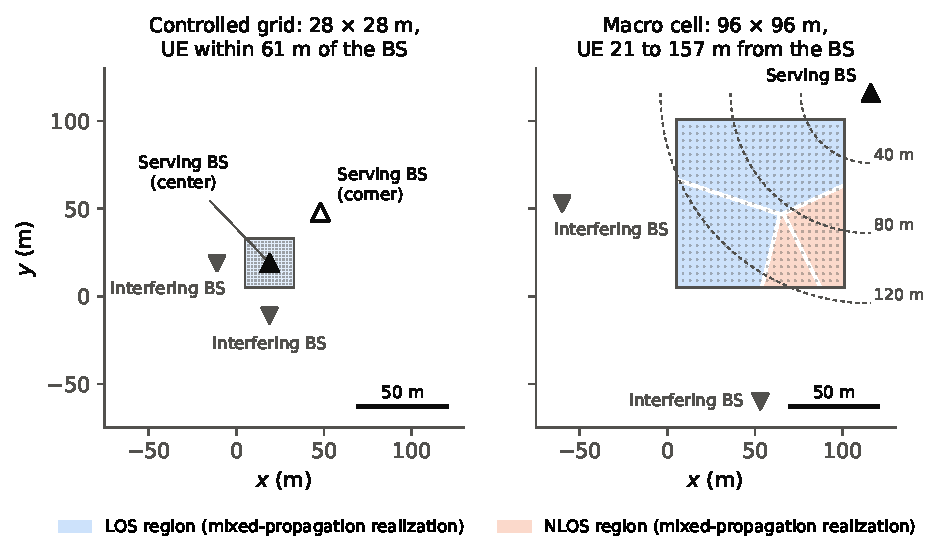
\includegraphics[width=0.95\textwidth]{fig_study_maps}
  \caption{The two deployments drawn at the same scale, with identical axes and a $50\,\text{m}$ scale bar in each panel. Left: the controlled grid, $15\times15$ cells at $2\,\text{m}$ pitch, with its two serving-BS placements~(filled: center; open: corner) and two interfering BSs. Right: the macro cell, $25\times25$ cells at $4\,\text{m}$ pitch, with the serving BS beyond its north-east corner, two interfering BSs, and range from the serving BS at $40$, $80$ and $120\,\text{m}$. Shading marks the macro cell's four Voronoi regions, park to the north and highway to the south-west~(LOS), shopping district to the south-east and residential area to the south~(NLOS), with the propagation each receives in the mixed-propagation realization; in the primary realization every region shares the same NLOS profile.}
  \label{fig:layout}
\end{figure}
% src: figure_scripts/make_figures.py study_maps(); grids, BS positions and Voronoi centres from the 15x15 and 25x25 configs; macro-cell transmitters from runners/run_multi_user_300_25x25.m (the 25x25 config's interferer entries, [-25,53] and [53,-25], are not used by that runner)

% src: configs/b6_los_blocked_los_config.jsonc (corridor length 200 m; strip widths 5-150 m; speeds 1.5, 4.0, 10.0 m/s; BS [100,500,10]; UMi LOS / UMi NLOS); CONTINUE_HERE.md §4 (360 users, constant-range rationale)
A fourth, targeted deployment, the \emph{blocked line-of-sight scenario}, follows UEs walking a straight $200\,\text{m}$ corridor whose middle section passes behind an obstruction, so that the link goes from LOS to NLOS and back. The width of the blocked strip is varied from $5$ to $150\,\text{m}$ and UE speed takes values of $1.5$, $4$ and $10\,\text{m/s}$. The BS stands $500\,\text{m}$ from the corridor so that range is nearly constant along it, which keeps the change in propagation from being confounded with a change in distance.

\subsection{Mobility}
\label{subsec:mobility}

% src: FINAL_REPORT.md §4.3
The controlled-grid study moves each UE on a random walk over the $8$-connected grid graph at $1.5\,\text{m/s}$; the walk carries no persistent heading. In the macro-cell study each user follows one of four trajectory patterns: straight-line navigation that reflects off the area boundary~($35\%$ of users), a random walk that continues straight with probability $0.7$~($35\%$), a tour between five sampled waypoints~($20\%$), or a straight transit across the area~($10\%$). Each user also belongs to one of four speed classes: pedestrian, $1.0$--$1.5\,\text{m/s}$~($40\%$); jogger, $2.5$--$4.5\,\text{m/s}$~($25\%$); vehicle, $8$--$15\,\text{m/s}$~($25\%$); or near-static, $0.1$--$0.5\,\text{m/s}$~($10\%$). All four patterns carry heading persistence, so the macro-cell mobility is favorable to history rather than adversarial to it.

% src: FINAL_REPORT.md §4.3, §5.8 (every step advances exactly one grid cell)
In both studies every step of a walk advances exactly one grid cell, and the time between snapshots is the step length divided by the UE's speed. A fixed history depth is therefore a fixed distance travelled, $h$ grid steps, but not a fixed duration: across the $232$ retained macro-cell users the time between snapshots $\Delta t$ ranges from $0.27$ to $32.5\,\text{s}$, with a median of $2.71\,\text{s}$. Position jitter of $\pm0.1\,\text{m}$ is added to every snapshot so that no estimator can latch onto exactly repeated coordinates.

\subsection{Device Model and AoA Impairment}
\label{subsec:device-model}

% src: FINAL_REPORT.md §4.4; technical_documentation.md §3.6, §3.7
The controlled-grid study simulates five device profiles: two four-antenna devices that differ only in their walk, a two-antenna device, a one-antenna device, and a two-antenna device carried at $0.9\,\text{m}$ height. The macro-cell study draws from a 3GPP-representative population of $85\%$ multi-antenna devices~(about $45\%$ with four antennas and $40\%$ with two) and $15\%$ single-antenna devices, each with its own antenna gain and carrying height. %TODO-CITE: 3GPP device-population mix assumption
Antenna count enters the channel through Equation~(\ref{eq:mrc}); the AoA capability of a device is then imposed when features are built, so the two device groups share an identical channel model and differ only in whether an angle is reported.

% src: FINAL_REPORT.md §4.4 (SINR-dependent model, controlled grid); csi_dataset.py load_and_prepare_data (macro cell: 4 deg Gaussian, 5 deg quantization, AoA = 0 for single-antenna devices)
Clean simulated arrival angles are degraded before use. In the controlled-grid study the noise on each axis depends on SINR,
\begin{equation}
  \sigma_{\text{AoA}}(t) = \operatorname{clamp}\!\left(2.0^\circ \cdot 10^{-\frac{\mathrm{SINR}_{dB}(t)-10}{15}},\ 1.0^\circ,\ 20.0^\circ\right),
  \label{eq:aoa-noise}
\end{equation}
while the macro-cell study applies a fixed $4^\circ$ Gaussian error, drawn independently for every report, an assumption that Section~\ref{subsec:averaging} shows to matter. Both then quantize azimuth and elevation to a $5^\circ$ codebook. Single-antenna devices cannot form a beam and report no angle; in the macro-cell features their angle is set to $0^\circ$.

\subsection{Features}
\label{subsec:features}

% src: technical_documentation.md §4.1-4.3
In the controlled-grid study, $\mathbf{m}(t)$ contains RSS and SINR, optionally extended with the AoA pair and with three device parameters: antenna count, antenna gain, and carrying height. The window of Equation~(\ref{eq:transition-history}) is built per user after sorting by time; the first $h$ snapshots of each user are dropped, and no window crosses from one user to another. Values are stacked in absolute form, because device-specific RSS and SINR offsets are stable across the grid and themselves act as fingerprints.

% src: FINAL_REPORT.md §4.5; csi_dataset.py build_derived_features (d_rss, d_az, d_ray_x, d_ray_y are per-user first differences divided by delta_t; ray = FSPL range estimate x AoA unit vector)
In the macro-cell study, each snapshot carries $13$ channels: RSS, SINR, the sines and cosines of both angles, which remove the $\pm180^\circ$ wrap discontinuity, two ray-projection coordinates formed from a path-loss range estimate and the AoA unit vector, the time increment $\Delta t$, and first differences of RSS, azimuth, and the two ray coordinates with respect to the previous snapshot, each divided by $\Delta t$. Every derived channel is computable from the raw measurements, so the derived set adds inductive bias rather than information. Because the first differences are part of each snapshot, the $h=0$ input of the macro-cell study already contains one step of change; it is the current snapshot together with its difference from the previous one, and the $h=5$ input stacks six such snapshots. Three static device features, antenna count, antenna gain, and carrying height, accompany every input.

\subsection{Estimators}
\label{subsec:estimators}

% src: CSI-Location experiments_ablation/model_zoo.py (build_classical, build_net, training constants); master_benchmark_rerun_summary.json (n_params)
The macro-cell study evaluates seven estimators spanning five algorithmic paradigms, listed in Table~\ref{tab:estimators}: $k$-nearest neighbors~($k$-NN), Random Forest, XGBoost, a gated recurrent unit~(GRU) network, and three one-dimensional convolutional neural networks~(1D-CNN), one with an AoA-validity channel and one with temporal self-attention. Hyperparameters are held fixed across history depths, so the input window is the only factor that varies within a model. The four neural models share a training recipe, AdamW at a learning rate of $3\times10^{-4}$ with weight decay $10^{-2}$, batch size $512$, a Huber loss on position with auxiliary speed and uncertainty heads, and at most $60$ epochs with early stopping. The controlled-grid study uses Random Forest and XGBoost classifiers, and its grid-size sweep adds a Gaussian likelihood model and a multilayer perceptron.

\begin{table}[h]
  \centering
  \caption{Estimators used in the macro-cell study.}
  \label{tab:estimators}
  \small
  \begin{tabular}{@{}lll@{}}
    \toprule
    Paradigm & Model & Configuration \\
    \midrule
    Instance-based & $k$-NN & $k=5$ \\
    Bagged trees & Random Forest & 150 trees, depth 16, min.\ leaf 5 \\
    Boosted trees & XGBoost & 50 trees, depth 5, learning rate 0.15 \\
    Recurrent & GRU & 2 layers, 254\,K parameters \\
    Convolutional & 1D-CNN & 3 convolutional layers, 67\,K parameters \\
    Convolutional & Mask-aware 1D-CNN & 1D-CNN with an AoA-validity channel, 67\,K parameters \\
    Attention & 1D-CNN with temporal self-attention & 200\,K parameters \\
    \bottomrule
  \end{tabular}
\end{table}

\subsection{Evaluation Protocol}
\label{subsec:protocol}

% src: FINAL_REPORT.md §4.7
The controlled-grid study splits each user's walk in time, training on the first $80\%$ of steps and testing on the last $20\%$; a random split would leak, because spatial consistency makes temporally adjacent samples near-duplicates. It is scored by exact-cell accuracy. The macro-cell study splits over users, so that the $47$ test users of each split are never seen during training, and it is scored by the 2D Euclidean error between predicted and true position: its mean, median, and 90th percentile, and the fraction of predictions within $5$, $10$ and $20\,\text{m}$. Every macro-cell result is reported separately for multi-antenna and single-antenna devices.

% src: seed_repeats_all_models.py docstring (seed drives split and init; marginal vs seed-paired)
The primary comparison is the change in error when history is added, measured within one model against its own $h=0$ input. For the macro-cell headline results the whole protocol is repeated over five seeds, each of which draws a different user split and model initialization. Two uncertainties follow. The marginal spread across seeds measures how much a single reported number could move by chance, and it is dominated by which users happen to land in the test set. The seed-paired difference compares two inputs on the same split and so cancels that source; it is the appropriate test for a change of input, and its $95\%$ confidence interval is reported with each gain.

% src: experiments_ablation/model_zoo.py train_deep docstring (early stopping on test MAE)
The neural models select their stopping epoch by error on the test users. This applies equally to both depths of a model, so within-model comparisons are unaffected, but it makes the absolute errors of the neural models, and any comparison between a neural model and a tree or instance-based model, optimistic in the neural model's favor.

\section{Results: The Controlled Grid}
\label{sec:results-controlled-grid}

% src: docs/results_of_record/controlled_grid_2026_10/{centre_bs,ne_bs}/results_summary.csv (regenerated 2026-10-13); technical_documentation.md §7.2.1, §7.3.2; constant-guess MAE 10.9 m from the test portion of the centre-BS data
Without AoA, adding three steps of history to RSS and SINR raised exact-cell accuracy in every configuration of the controlled-grid study, for both classifiers and both BS placements~(Figure~\ref{fig:cg-placement}). With the BS at the center, XGBoost gained $14.4$ percentage points ($13.8\%$ to $28.2\%$) and Random Forest $11.7$ ($22.7\%$ to $34.3\%$); with the BS beyond the corner they gained $13.3$ ($11.3\%$ to $24.7\%$) and $9.7$ points ($18.8\%$ to $28.5\%$). Mean position error fell by $2.5$ to $3.2\,\text{m}$ in all four cases, between $27\%$ and $33\%$. These snapshot models are weak: always guessing the center of the grid gives a mean error of $10.9\,\text{m}$ on the test samples, and without history XGBoost reaches $10.4\,\text{m}$ and Random Forest $9.2\,\text{m}$ at the center. History therefore lifts RSS and SINR from a level close to the trivial guess to a modest one, and the gain is of similar size for both classifiers and both placements.

\begin{figure}[h]
  \centering
  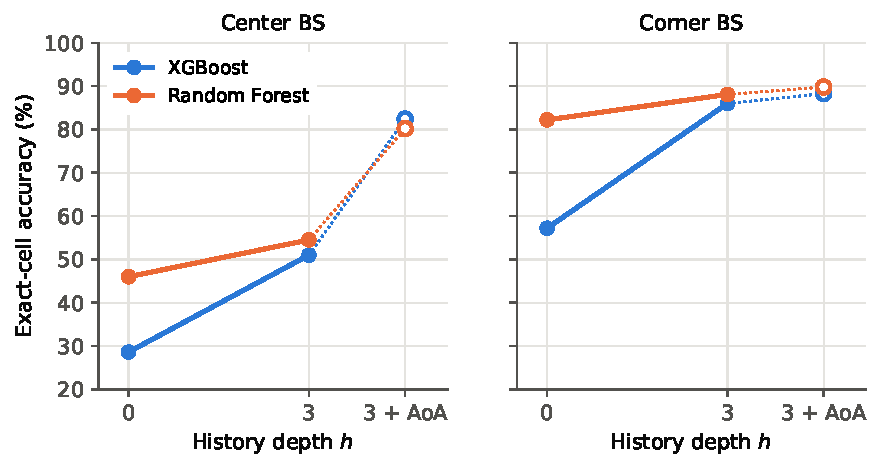
\includegraphics[width=0.85\textwidth]{fig_controlled_grid_placement}
  \caption{Controlled grid: exact-cell accuracy from RSS and SINR, and with AoA added, at history depth $h=0$ and $h=3$, with the BS at the grid center~(left) and beyond its corner~(right). Single run per configuration, simulated at $3.5\,\text{GHz}$ with one urban-micro NLOS propagation scenario for every walk.}
  \label{fig:cg-placement}
\end{figure}
% src: technical_documentation.md §7.2.1, §7.3.1, §7.3.3; figure_scripts/make_figures.py controlled_grid_placement()

% src: results_of_record/controlled_grid_2026_10 results_summary.csv (BASE_H3 vs BASE_A_H3); technical_documentation.md §7.3.1
The same placement change that leaves history's contribution positive removes most of AoA's. With history already in the input, adding AoA raised XGBoost's accuracy by $39.2$ points at the center BS but by $6.2$ points at the corner, and Random Forest's by $33.0$ and $5.8$ points. From the corner the whole grid falls within a wedge of about $52^\circ$, and once a $5^\circ$ codebook and a few degrees of estimation noise are applied, azimuth no longer separates neighboring cells; with AoA and history the corner placement reaches only $30.9\%$ for XGBoost against $67.5\%$ at the center. The remaining gain at the corner is consistent with elevation, which encodes distance, but this grid study does not isolate it. This loss of AoA's value is specific to a short-range grid with $2\,\text{m}$ cells; it is not a general property of corner placements.

% src: FINDINGS.md §3.3 (7x7, RSS+SINR, raw stacking: XGB 26.8/38.7/43.5/45.4; RF 28.0/38.3/42.6/43.6; MLP 24.8/36.9/38.6/41.6); analysis/regression_vs_classification.md §4.1-4.2 (15x15 single scenario with AoA: UMa NLOS 29.18/46.12/49.48/51.23; UMa LOS 92.59/95.90/95.54/95.86)
Where history was swept one step at a time, most of the gain arrived with the first step~(Figure~\ref{fig:cg-depth}). On a single-user $7\times7$ grid, one step of history raised accuracy by $10$ to $12$ points for each of XGBoost, Random Forest and a multilayer perceptron, and the next two steps added about $5$ to $7$ points between them. With AoA available, the same profile appears in a uniform urban-macro NLOS scenario, where accuracy rose from $29\%$ to $46\%$ at the first step and to $51\%$ by $h=3$. In the corresponding LOS scenario, where AoA alone already placed $93\%$ of samples in the right cell, history added $3$ points at the first step and nothing after it.

\begin{figure}[h]
  \centering
  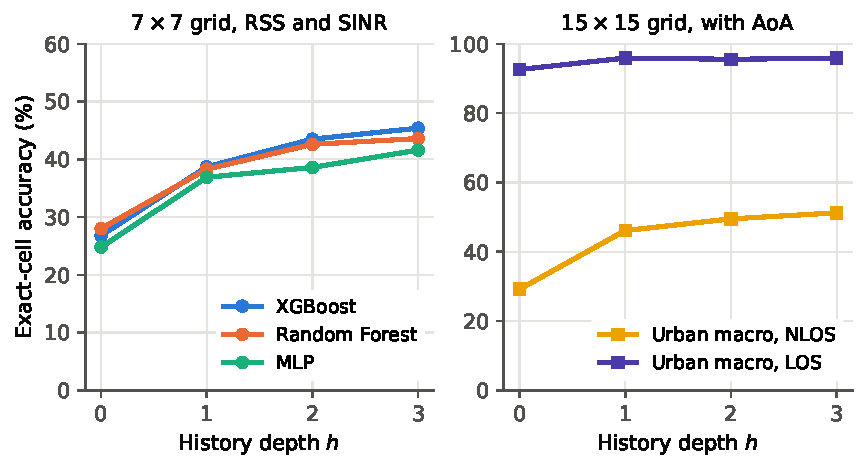
\includegraphics[width=0.85\textwidth]{fig_controlled_grid_depth}
  \caption{Controlled grid, single user: exact-cell accuracy as history depth grows. Left: $7\times7$ grid with RSS and SINR, three classifiers. Right: $15\times15$ grid with AoA in a single urban-macro propagation scenario, NLOS and LOS. Single run per point.}
  \label{fig:cg-depth}
\end{figure}
% src: figure_scripts/make_figures.py controlled_grid_depth()

% src: technical_documentation.md §7.1 (grid sweep, single user, XGBoost); §7.1 second table (7x7, four algorithms)
The direction of the history effect is also stable across scale and estimator~(Figure~\ref{fig:cg-scale}). In the single-user version of the study, history raised accuracy at every grid size from $3\times3$ to $20\times20$ cells, by between $9.2$ and $21.8$ points, and on the $7\times7$ grid it raised the accuracy of all four estimators tried, from $4.7$ points for a Gaussian likelihood model to $18.2$ points for XGBoost.

\begin{figure}[h]
  \centering
  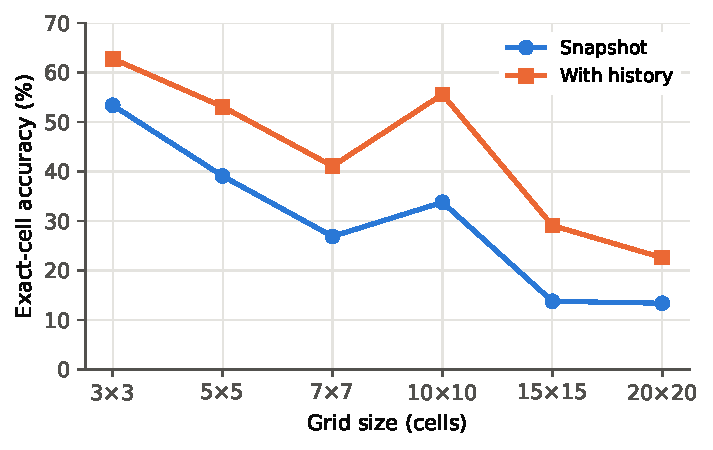
\includegraphics[width=0.65\textwidth]{fig_controlled_grid_scale}
  \caption{Controlled grid, single user: exact-cell accuracy with and without history as the grid grows from $3\times3$ to $20\times20$ cells, XGBoost with RSS and SINR at the best depth up to $h=3$. Single run per grid size.}
  \label{fig:cg-scale}
\end{figure}
% src: technical_documentation.md §7.1; figure_scripts/make_figures.py controlled_grid_scale()

% src: results_of_record/controlled_grid_2026_10/centre_bs/results_summary.csv (BASE_dp 25.88/30.58 -> BASE_H3_dp 33.75/39.72; BASE_A_dp 65.41/67.26 -> BASE_A_H3_dp 68.42/67.85); technical_documentation.md §7.2.6
Because RSS and SINR are stacked in absolute form, part of what a history window carries is a stable, device-specific offset, and history could in principle be helping only by identifying the device. Supplying the device parameters directly rules this out as the whole story: with antenna count, gain and height already in the input, history still added $7.9$ points for XGBoost and $9.1$ for Random Forest at the center BS. The device parameters themselves are worth about as much as history ($12.0$ and $7.9$ points over the snapshot model), and the user identifier alone is as informative as the parameters, so their gain is a device-identity effect. With AoA available at the center BS, history added less, $3.0$ points for XGBoost and $0.6$ for Random Forest on top of the device parameters, since a classifier that already reaches about $65\%$ from AoA has less ambiguity left for history to resolve.

% src: earlier pair of runs of the same configuration (technical_documentation.md history; superseded data) differed by 2-3 points; the controlled-grid runs were regenerated 2026-10-13 (RESULTS_DIRECTORY_MAP.md §7)
Every number in this section comes from a single run, and the same configuration evaluated in two separate runs differed by $2$ to $3$ points in an earlier version of this study, so only differences well above that are read as effects. The depth and scale sweeps above come from earlier single-user simulations that were not regenerated. The controlled grid also tests later time steps of users seen in training, at no more than $61\,\text{m}$ from the BS. Whether history keeps its value at macro-cell range, for users the model has never seen and a population with mixed hardware, is the question the macro-cell study answers.

\section{Results: What Accuracy a Macro Cell Allows}
\label{sec:results-error-scale}

% src: FINAL_REPORT.md §7.5 (pooled fit gamma 3.26, sigma 10.11 dB, R^2 0.204); pathloss_fit_summary.json comparison (fitted_gamma 3.264, fitted_sigma_db 10.106) and range_resolution (sigma_r 40.14 / 67.94 / 89.97 m at 56 / 95 / 126 m; 7.13 m at 10 m)
At the distances of the macro-cell study, RSS alone pins down range only to within tens of meters, and that sets the scale against which every error in the following sections should be read. Fitting Equation~(\ref{eq:path-loss}) to all $144{,}437$ macro-cell snapshots, with the antenna gain and antenna count of each device as controls, gives $\gamma = 3.26$ and a residual shadowing spread of $\sigma = 10.1\,\text{dB}$; range explains only $20\%$ of the variance in RSS. Dividing $\sigma$ by the gradient of Equation~(\ref{eq:rss-gradient}) turns this into the range uncertainty $\sigma_r$ implied by a single RSS reading: $40\,\text{m}$ at the 10th percentile of macro-cell range~($56\,\text{m}$), $68\,\text{m}$ at the median~($95\,\text{m}$), and $90\,\text{m}$ at the 90th percentile~($126\,\text{m}$). The same calculation gives $7\,\text{m}$ at $10\,\text{m}$ from the BS, the distance typical of the controlled grid. The two studies therefore differ not only in size but in how much a single RSS value says about distance, by roughly an order of magnitude. This is a ranging resolution and not a baseline: a model that ignored every measurement and always predicted the mean training position would be wrong by about $35\,\text{m}$ (Table~\ref{tab:reference-levels}).

Table~\ref{tab:reference-levels} sets this physical reference beside measured errors for both device groups, and beside the error of the simplest possible predictor, which always returns the mean training position: $35.3\,\text{m}$ for multi-antenna devices and $38.5\,\text{m}$ for single-antenna devices. A snapshot $k$-NN fingerprint, the classical approach, misses multi-antenna devices by $23\,\text{m}$ on average and single-antenna devices by $46\,\text{m}$, which for single-antenna devices is worse than the constant guess. The trained models do considerably better for multi-antenna devices: over $20$ user splits XGBoost is $47\%$ below the constant guess at $h=0$ and $56\%$ below it at $h=5$. For single-antenna devices they do not: XGBoost is $6\%$ below it at $h=0$ and $5\%$ at $h=5$, and the two groups remain about $20\,\text{m}$ apart in every model.

\begin{table}[h]
  \centering
  \caption{Reference error levels in the macro-cell study, per device group. Measured errors are means over five seeds, and the constant-guess errors means over $20$ seeds; neural-model errors are optimistic because their stopping epoch was chosen on the test users. The ranging resolution is a standard deviation, not an error.}
  \label{tab:reference-levels}
  \small
  \begin{tabular}{@{}lrr@{}}
    \toprule
    Reference & Multi-antenna & Single-antenna \\
    \midrule
    Constant guess (mean training position) & $35.3\,\text{m}$ & $38.5\,\text{m}$ \\
    RSS ranging resolution $\sigma_r$ at median range & $68\,\text{m}$ & $68\,\text{m}$ \\
    \midrule
    $k$-NN, $h=0$ & $23.4\,\text{m}$ & $46.2\,\text{m}$ \\
    XGBoost, $h=0$ & $18.8\,\text{m}$ & $35.8\,\text{m}$ \\
    XGBoost, $h=5$ & $15.7\,\text{m}$ & $35.8\,\text{m}$ \\
    Best of seven models, $h=5$ & $15.5\,\text{m}$ & $34.5\,\text{m}$ \\
    \bottomrule
  \end{tabular}
\end{table}
% src: constant guess: followup_2026_10/naive_baseline/*/naive_position_baseline_summary.json (20 seeds: multi 35.27+-0.54, single 38.50+-1.21, all 35.67); XGBoost vs guess: followup_2026_10/uniform_nlos snap/full means 18.74/15.59 multi, 36.33/36.51 single; row 2 as above; rows 3-6: seed_repeats_all_models_summary.json per_config (knn_h0 23.38/46.17; xgboost_h0 18.81/35.84; xgboost_h5 15.65/35.77; best h5: cnn_attn multi 15.45, mask_aware_cnn single 34.52)

% src: diagnostics_2026_10/baseline_uniform_nlos summary per_seed.xgboost.{snap,full} (5 seeds): within_5m/10m/20m, p50, p90; errors_first_seed.npz (figure, seed 42)
The two groups are clearly separated in the error distribution, though not disjoint~(Figure~\ref{fig:error-cdf}): their error histograms overlap by $52\%$ with history and $63\%$ without in the plotted split. With five steps of history, XGBoost places $34\%$ of multi-antenna predictions within $10\,\text{m}$ of the true position and $71\%$ within $20\,\text{m}$, with a median error of $13.7\,\text{m}$ and a 90th percentile of $29.5\,\text{m}$. For single-antenna devices the corresponding fractions are $7\%$ and $21\%$, the median is $34.7\,\text{m}$, and the 90th percentile is $59.1\,\text{m}$. Fewer than $12\%$ of multi-antenna predictions and $2\%$ of single-antenna predictions fall within $5\,\text{m}$.

\begin{figure}[h]
  \centering
  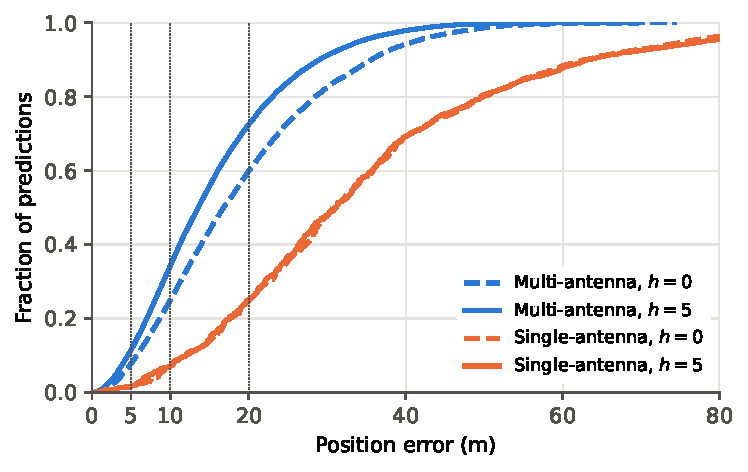
\includegraphics[width=0.7\textwidth]{fig_error_cdf}
  \caption{Distribution of position error per device group, XGBoost without history~($h=0$, dashed) and with five steps of history~($h=5$, solid), macro-cell study, one seed. Dotted lines mark $5$, $10$ and $20\,\text{m}$.}
  \label{fig:error-cdf}
\end{figure}
% src: figure_scripts/make_figures_diagnostic.py error_cdf(); diagnostics_2026_10/baseline_uniform_nlos/errors_first_seed.npz

% src: diagnostics_2026_10/baseline_uniform_nlos summary per_seed.xgboost.{snap,full} radial_mean / tangential_mean (5-seed means: multi h5 14.12 / 4.60; single h5 20.13 / 25.29); radial share = r^2/(r^2+t^2) as in error_decomposition.py; followup_2026_10/uniform_nlos summary.xgboost.snap.single.shape (20 seeds: radial share 0.41+-0.02, range_corr 0.51+-0.06, radial_bias -9.73) and full.multi.shape radial_rms 17.45
The two groups also fail in different directions. Splitting each error into its component along the line to the BS, the radial or range error, and the component across it, the tangential or cross-range error, shows that multi-antenna devices are limited by range. With history, their mean radial error is $14.1\,\text{m}$ against a tangential error of $4.6\,\text{m}$, so $90\%$ of their error variance lies along the line to the BS. That radial error, $17.5\,\text{m}$ in root-mean-square terms, is about four times smaller than the $68\,\text{m}$ standard deviation of a single-reading range estimate, so the models extract considerably more range information than a path-loss inversion. Single-antenna devices fail differently. Their tangential error of $25.3\,\text{m}$ exceeds their radial error of $20.1\,\text{m}$, and about $60\%$ of their squared error is tangential, which is the distance-ring ambiguity of Section~\ref{subsec:ambiguity-hypothesis} observed. But they are not placed at the right distance: their radial error is larger than that of multi-antenna devices, the predicted range correlates only $0.51 \pm 0.06$ with the true range, and predictions are pulled toward the BS by about $10\,\text{m}$ on average. Over $20$ splits these devices are only $5$ to $6\%$ better than the constant guess of Table~\ref{tab:reference-levels}.

% src: diagnostics_2026_10/baseline_uniform_nlos summary per_seed.xgboost.{snap,full}.groups.*.range_bins (5-seed means; multi h0 21.3/21.2/14.5/28.6, h5 11.1/17.2/12.9/23.1; single h0 31.9/30.4/37.5/41.0; mean test samples per band, single: 163/1318/2549/728)
Error does not simply grow with distance from the BS~(Figure~\ref{fig:error-by-range}). For multi-antenna devices the band from $80$ to $120\,\text{m}$, which holds about half of the test samples, has the smallest error, while both the nearest band and the farthest have larger errors. The nearest band is also where history makes the largest difference, cutting the mean error from $21.3$ to $11.1\,\text{m}$. Single-antenna error rises from about $30\,\text{m}$ within $80\,\text{m}$ of the BS to about $40\,\text{m}$ beyond $120\,\text{m}$, and history changes it in none of the bands. Only about $160$ single-antenna test samples per split fall within $40\,\text{m}$ of the BS, so that band is the least certain.

\begin{figure}[h]
  \centering
  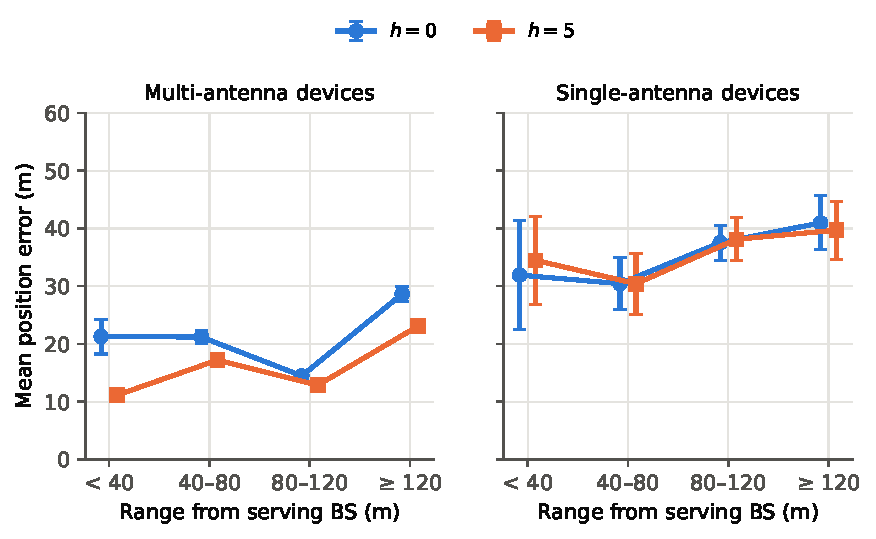
\includegraphics[width=0.85\textwidth]{fig_error_by_range}
  \caption{Mean position error by range from the serving BS, per device group, XGBoost without and with history, macro-cell study. Means over five seeds; bars are $95\%$ confidence intervals across seeds.}
  \label{fig:error-by-range}
\end{figure}
% src: figure_scripts/make_figures_diagnostic.py error_by_range()

% src: FINAL_REPORT.md §7.5 ("eight differences": 784 vs 9,216 m^2; ~1,600 vs 178 samples per cell; seen vs unseen users)
The gap between the controlled grid's sub-meter errors and the macro cell's tens of meters follows from these references rather than from a failure of the models. Beyond the order-of-magnitude difference in what one RSS reading says about range, the macro cell covers twelve times the area, offers about nine times fewer training samples per grid cell, and tests on users the model has never seen. Because the two device groups fail in such different ways, the effect of history has to be measured on each of them separately.

\section{Results: Multi-Antenna Devices}
\label{sec:results-multi}

% src: seed_repeats_all_models_summary.json per_config.*_h0/_h5 runs (seed-paired multi_mae differences, computed per seed; CI = 1.96 sd / sqrt(5))
For multi-antenna devices, history lowered error in every one of the seven model families, by $2.8$ to $4.1\,\text{m}$, or $15$ to $21\%$ of each model's own $h=0$ error~(Figure~\ref{fig:history-gain-ci}; per-model values in Table~\ref{tab:history-gain}). Each gain is a seed-paired difference over five independent user splits, and none of the seven confidence intervals comes close to zero. The gain is of similar size across instance-based, bagged, boosted, recurrent, convolutional and attention-based models, which is the behavior expected if history supplies information that the $h=0$ input lacks, rather than suiting one architecture's inductive bias. These gains are measured under the angle impairment of Section~\ref{sec:setup}, in which every report carries an independent $4^\circ$ error; Section~\ref{subsec:averaging} shows how much of the gain depends on that.

\begin{figure}[h]
  \centering
  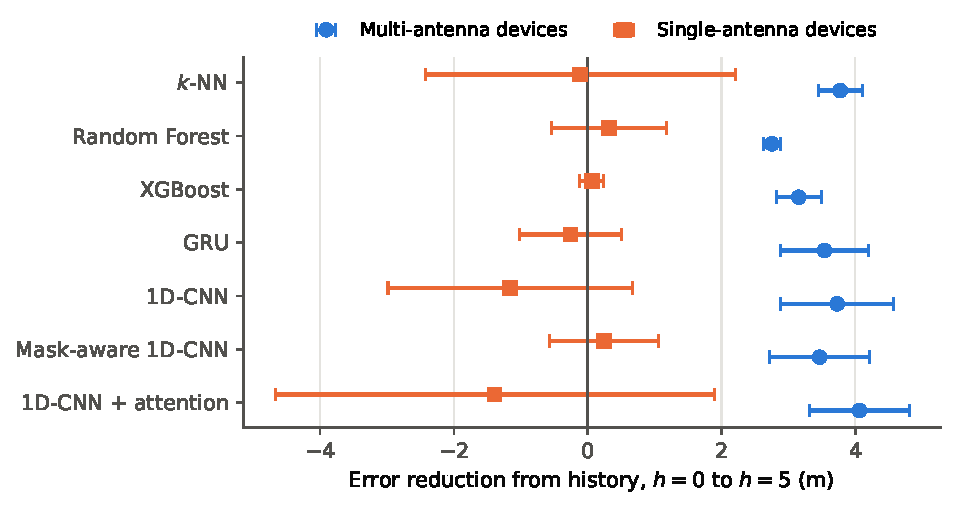
\includegraphics[width=0.8\textwidth]{fig_history_gain_ci}
  \caption{Reduction in mean error from adding history~($h=0$ to $h=5$), per model and device group, macro-cell study. Each marker is the mean seed-paired difference over five user splits; bars are $95\%$ confidence intervals. Positive values mean history lowered the error.}
  \label{fig:history-gain-ci}
\end{figure}
% src: figure_scripts/make_figures.py history_gain_ci(); seed_repeats_all_models_summary.json

% src: history_sweep_all_models_summary.json curves (seed 42, multi_mae by depth)
The gain builds over the first few steps of history and then levels off~(Figure~\ref{fig:history-by-group}, left). With the exception of $k$-NN, whose error rises again between $h=5$ and $h=10$, and Random Forest, which is flat over that interval, every family is still improving at $h=10$, or $40\,\text{m}$ of travel. For XGBoost the overall error varies by only about $0.05\,\text{m}$ between $h=10$ and $h=30$. In follow-up runs over $10$ to $20$ user splits, XGBoost's gain from the full window is $1.2$, $2.5$, $3.2$, $3.5$ and $3.7\,\text{m}$ at $1$, $3$, $5$, $10$ and $20$ steps, so most of it is in place by $10$ steps. No single depth is optimal across families; what distinguishes them is whether an over-long window costs anything. A tree ensemble can decline to split on an uninformative lag, whereas $k$-NN measures distance over the whole concatenated window, so each stale lag adds noise to its metric; this account is offered as an interpretation of the depth curves rather than as a separately tested result.
% src: deep_history_sweep_trees_summary.json (XGBoost h=10..30 spread 0.053 m); FINAL_REPORT.md §5.4

\begin{figure}[h]
  \centering
  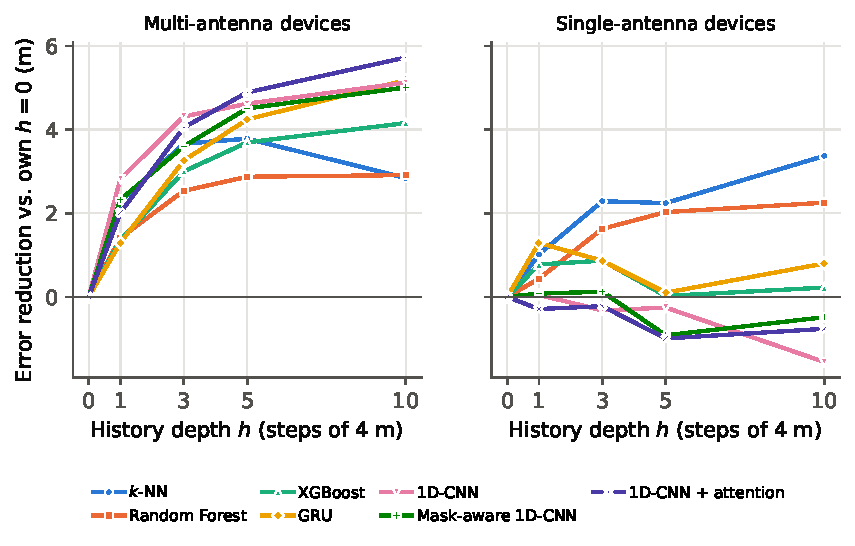
\includegraphics[width=0.9\textwidth]{fig_history_by_group}
  \caption{Error reduction against each model's own $h=0$ input as history depth grows, macro-cell study. Each step of history is $4\,\text{m}$ of travel. Single seed; the single-antenna curves move within that group's seed-to-seed spread, and the five-seed paired values at $h=5$ are those of Figure~\ref{fig:history-gain-ci}.}
  \label{fig:history-by-group}
\end{figure}
% src: figure_scripts/make_figures.py history_by_group(); history_sweep_all_models_summary.json

% src: history_by_speed_class_summary.json by_model.cnn (seed 42; best h 10/10/5/5 for static/pedestrian/jogger/vehicle; windows 134.7/31.0/7.1/1.6 s); FINAL_REPORT.md §5.8 (7-18 test users per class)
Because each step covers one grid cell, history depth measures distance travelled rather than elapsed time, and the speed classes of the population separate the two~(Figure~\ref{fig:speed-classes}). Measured against path length, the four classes improve over a similar span: every class has gained most of its benefit within $12$ to $20\,\text{m}$. Measured against time, the same curves are spread across two orders of magnitude, and the 1D-CNN's best window lasts $1.6\,\text{s}$ for vehicles but $135\,\text{s}$ for near-static users. The useful window is therefore set by how far a device has moved through the spatially consistent channel, not by how long it took to do so. Vehicles gain least, about $4\%$ against $17$ to $28\%$ for the other classes. Each class contains only $7$ to $18$ test users, so these are single-seed indications, and because step length is fixed in these simulations, the number of samples and the distance covered cannot be separated.

\begin{figure}[h]
  \centering
  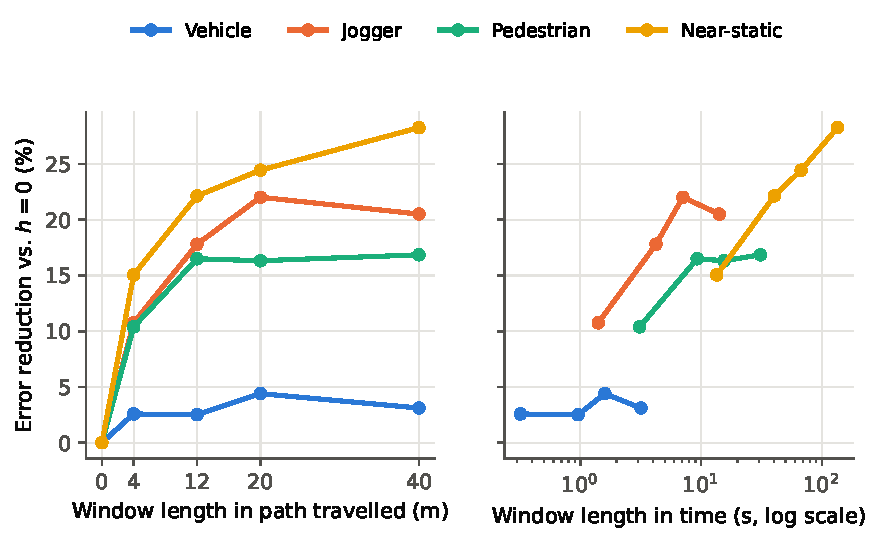
\includegraphics[width=0.85\textwidth]{fig_speed_classes}
  \caption{Error reduction against $h=0$ for each speed class, 1D-CNN, macro-cell study, plotted against the window's length in path travelled~(left) and in time~(right, logarithmic). Points correspond to $h=0$, $1$, $3$, $5$ and $10$. Single seed, $7$ to $18$ test users per class.}
  \label{fig:speed-classes}
\end{figure}
% src: figure_scripts/make_figures.py speed_classes()

% src: xgb_per_h_retune_summary.json and rf_per_h_retune_summary.json: XGBoost tuning buys <= 0.44 m; RF tuning moves -0.046 to +0.066 m
Two checks rule out the most direct alternative explanations. A larger input could help simply because fixed hyperparameters happen to suit it better, so XGBoost and Random Forest were re-tuned separately at every depth, on training users only. Re-tuning changed XGBoost's error by at most $0.44\,\text{m}$ and Random Forest's by less than $0.07\,\text{m}$, and the history gain was essentially unchanged~(Table~\ref{tab:supp-retune}). The derived input channels also matter less than history: replacing them with the five raw channels raised the 1D-CNN's error at $h=5$ by $0.43\,\text{m}$ in a single run, a difference that is suggestive but small beside the gain from history.
% src (feature ablation): FINAL_REPORT.md §5.2 (19.686 raw vs 19.260 derived, 1D-CNN, h=5)

% src: seed_repeats_all_models_summary.json ranking (h=5 overall, ranks 1-6 18.810-19.275, all adjacent pairs overlapping); master_benchmark_rerun_summary.json (cost)
With history in place, the choice of model matters far less than the input. At $h=5$ the six trained models other than $k$-NN fall within $0.47\,\text{m}$ of each other in overall error, with overlapping confidence intervals for every adjacent pair. XGBoost reaches that level in $4\,\text{s}$ of training and predicts $1000$ positions in a few milliseconds ($1.7\,\text{ms}$ in one timing and $8.3\,\text{ms}$ in another), and the neural models' errors are, if anything, flattered by their test-based stopping rule. A small boosted-tree ensemble therefore collects the full benefit of history at a fraction of the cost.

% src: rts_retune_all_models_summary.json (best RTS gains: RF 2.49, XGB 4.35, 1D-CNN 3.65, GRU 3.72, attention 4.74%); trajectory_diagnostics_summary.json via FINAL_REPORT.md §7.7 (forward Kalman 19.13 -> 19.77 m, 1D-CNN)
Temporal information can also be used after the estimator rather than inside it. A Rauch--Tung--Striebel~(RTS) smoother applied to the trained models' predicted tracks lowered their error by a further $2.5$ to $4.7\%$, but with two qualifications: the smoother's noise parameters were tuned on the test users, and its gain comes entirely from the backward pass, which uses future samples. Running only the forward filter raised the 1D-CNN's error by $3.4\%$. Smoothing is thus a complement to history for offline track reconstruction, whereas history uses past samples only and is available in real time.

% Hand-off to the single-antenna section
All of these gains belong to devices that report an angle. Single-antenna devices are the ones that face the distance-ring ambiguity in its pure form, and they are where history would be expected to matter most.

\section{Results: Single-Antenna Devices}
\label{sec:results-single}

% src: seed_repeats_all_models_summary.json per_config.*_h0/_h5 runs (seed-paired single_mae differences)
For single-antenna devices in the macro-cell study, history produced no detectable change in error in any of the seven model families~(Figure~\ref{fig:history-gain-ci}). The seed-paired changes from $h=0$ to $h=5$ range from a $1.39\,\text{m}$ increase to a $0.32\,\text{m}$ decrease, and every confidence interval spans zero. The null result is tight where the measurement is precise: XGBoost's change is $0.06 \pm 0.18\,\text{m}$ on a baseline of $35.8\,\text{m}$, and Random Forest's is $0.32 \pm 0.86\,\text{m}$. The same seven models gained $15$ to $21\%$ on multi-antenna devices drawn from the same test users. Each split contains between $5$ and $10$ single-antenna test users, eight on average, which is why their confidence intervals are wider. With $50\%$ of the devices single-antenna, which gives $14$ to $22$ such test users per split, XGBoost shows a small gain after all, $0.30 \pm 0.24\,\text{m}$, and Random Forest none, $0.18 \pm 0.24\,\text{m}$. The accurate statement is that history gives these devices no more than about $1\%$ on uniform-NLOS data.
% src: diagnostics_2026_10/*/history_mechanism_diagnostic_summary.json user_counts (single-antenna test users per seed 42/1/7/13/99: 10, 7, 6, 10, 5; identical splits in both datasets)

% src: FINAL_REPORT.md §7.3 (outlier audit, 1D-CNN, single run: worst five all 1-antenna, best five all multi-antenna; user 250 raw MAE 33.84 m, Figure 6); diagnostics_2026_10/baseline_uniform_nlos/errors_first_seed.npz (seed 42, XGBoost: user 250 true bearing span 73 deg, predicted 17 deg at h=0 and h=5, range mean 94/96 vs 103 true; user 27 span 65 vs 68 deg); followup_2026_10/naive_baseline; single_share_50/uniform_nlos
The reason is visible in Section~\ref{sec:results-error-scale}: always predicting the mean training position gives $38.5\,\text{m}$ for these devices, so a snapshot model at $36.3\,\text{m}$ has recovered only about $6\%$ of it, and history leaves that unchanged. Figure~\ref{fig:trajectories} shows what the failure looks like for the median single-antenna test user. The user's walk spans $73^\circ$ of bearing, but the predicted positions, with or without history, span only $17^\circ$, at roughly the right distance from the BS (mean predicted range $96\,\text{m}$ against $103\,\text{m}$ true). This user is illustrative; over all single-antenna devices the predicted range correlates only $0.51$ with the true range. The median multi-antenna user's predictions instead follow the shape of the walk, spanning $68^\circ$ against $65^\circ$ true. This pattern dominates the tail of the error distribution: in a single-run audit of every test user, all five users with the largest error were single-antenna devices and all five with the smallest were multi-antenna devices.
% src: FINAL_REPORT.md §7.3 (outlier audit, 1D-CNN, single run)

\begin{figure}[h]
  \centering
  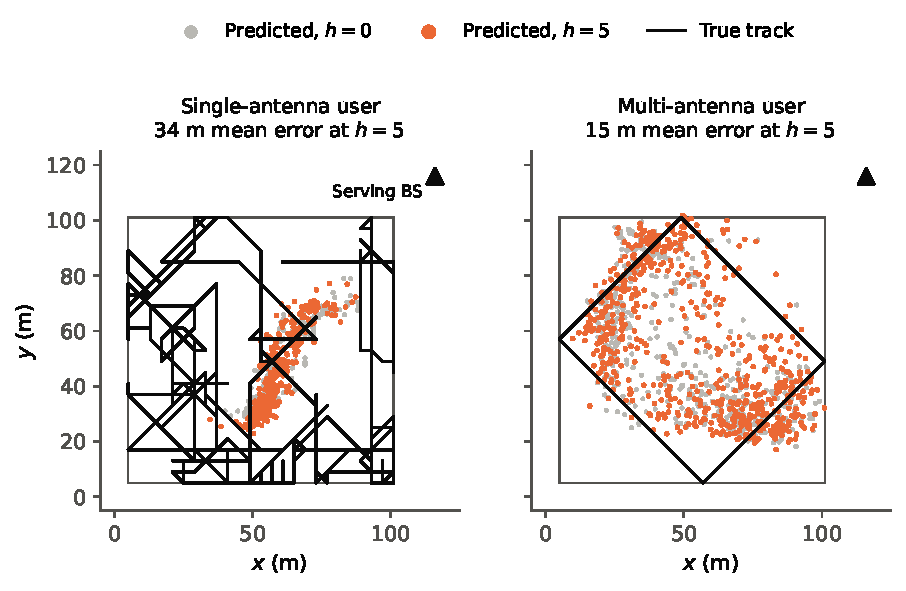
\includegraphics[width=0.92\textwidth]{fig_trajectories}
  \caption{True track and predicted positions of the median single-antenna~(left) and median multi-antenna~(right) test user, ranked by error at $h=5$. XGBoost without history~(gray) and with five steps of history~(orange), macro-cell study, one seed. The box marks the grid; the triangle marks the serving BS.}
  \label{fig:trajectories}
\end{figure}
% src: figure_scripts/make_figures_diagnostic.py trajectories(); diagnostics_2026_10/baseline_uniform_nlos/errors_first_seed.npz (seed 42; users 250 and 27, mean error at h=5 33.9 and 15.0 m)

% src: technical_documentation.md §7.4.1 (untuned, spherical: RF BASE 15.243 -> BASE_H3 18.057), §7.4.3 (tuned Cartesian: RF 14.022 -> 16.272; XGB 29.239 -> 13.430), §7.4.4 (block-shuffled: RF 13.811 -> 17.342; XGB 29.766 -> 14.800)
The single-user $25\times25$ regression runs point the same way at the same range, under a different split~(Figure~\ref{fig:single-user}). With RSS and SINR only, Random Forest's error rose when three steps of history were added, from $14.0$ to $16.3\,\text{m}$ under a chronological split and from $13.8$ to $17.3\,\text{m}$ when the walk was cut into shuffled five-step blocks to prevent any memorization of the path. XGBoost's error fell sharply with history in the same runs, but only from a snapshot model that was about twice as poor as Random Forest's, to roughly Random Forest's snapshot level. In none of these runs did a model with RSS and SINR history beat the best snapshot model by a margin worth reporting. Random Forest's loss is consistent with a feature-subsampling effect: replacing the stacked absolute lags with differences from the current snapshot removed it in a related configuration with AoA, and the macro-cell features already include such differences.
% src: technical_documentation.md §7.4.5 (hybrid delta features: RF 8.090 -> 7.636 m)

\begin{figure}[h]
  \centering
  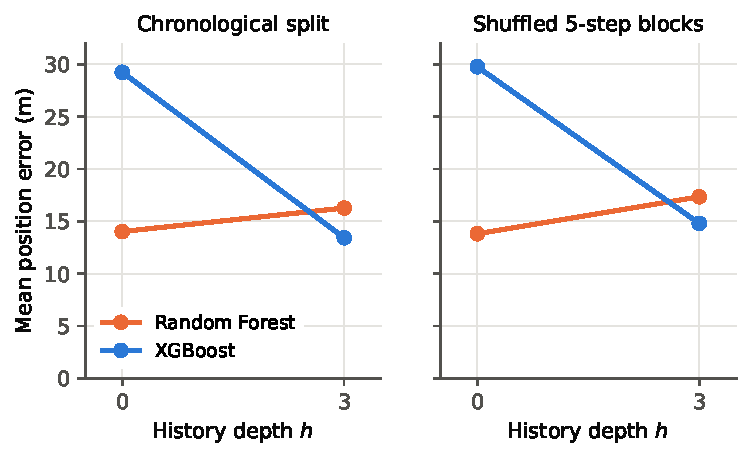
\includegraphics[width=0.7\textwidth]{fig_single_user_no_aoa}
  \caption{Single-user $25\times25$ regression with RSS and SINR only: mean position error without history and with three steps of history, under a chronological split~(left) and with the walk cut into shuffled five-step blocks~(right). Single run per point.}
  \label{fig:single-user}
\end{figure}
% src: figure_scripts/make_figures.py single_user_no_aoa(); technical_documentation.md §7.4.3, §7.4.4

% src: FINAL_REPORT.md §7.6 (1D-CNN masking: single 33.607 -> 32.188, multi 15.408 -> 15.279), §7.6.1 (k-NN/RF/XGB single: 39.968 -> 40.295, 33.069 -> 33.145, 34.806 -> 34.492; overall worse in all three); §5.7 significance table
How a missing angle is encoded does matter for one kind of model. Feeding single-antenna devices a dummy $0^\circ$ angle makes the derived channels assert a confident bearing, since $\cos 0^\circ = 1$. Replacing the angle embeddings with zeros, a point off the unit circle that no real angle can produce, and adding an explicit flag for angle validity lowered the 1D-CNN's single-antenna error from $33.6$ to $32.2\,\text{m}$ in a paired single-seed comparison, with a negligible $0.13\,\text{m}$ change for multi-antenna devices. The same encoding did not help $k$-NN, Random Forest or XGBoost, whose overall error rose slightly in all three cases. A tree can already branch on antenna count and ignore the angle channels when they carry nothing, whereas a convolution applies the same filters to every sample and cannot. The $1.4\,\text{m}$ improvement exceeds the paired uncertainty of the history comparison but lies within the seed-to-seed spread of the single-antenna error, so it is suggestive rather than established.

\subsection{A Range-Dependent Explanation}
\label{subsec:hypothesis}

% src (derived): pathloss_fit_summary.json range_resolution fitted_db_per_m (1.4176 dB/m at 10 m; 0.1487 dB/m at 95 m) x step length (2 m controlled grid; 4 m macro cell); sigma 10.1 dB; angular: 4 m / 95 m rad = 2.4 deg vs 4 deg Gaussian + 5 deg codebook (csi_dataset.py)
The contrast with the controlled grid, where RSS and SINR history did help, has a candidate explanation in Equation~(\ref{eq:rss-gradient}). Without an angle, a history window can only reveal motion through changes in RSS and SINR, and the change produced by one step shrinks with distance from the BS. With the fitted constants, a $2\,\text{m}$ step at $10\,\text{m}$ from the BS changes RSS by about $2.8\,\text{dB}$, whereas a $4\,\text{m}$ step at the macro cell's median range of $95\,\text{m}$ changes it by about $0.6\,\text{dB}$, almost five times less, against shadowing with a spread of $10\,\text{dB}$. An angle measurement weakens with range too, but far less severely relative to its noise: a $4\,\text{m}$ sideways step at $95\,\text{m}$ turns the bearing by about $2.4^\circ$, comparable to the $4^\circ$ angle error. On this account, history helps wherever the step-to-step change in some measured channel stands out from that channel's noise, which at macro range is true of the angle channels and not of RSS.

The account is a hypothesis. The controlled grid and the macro cell differ in other ways as well, most notably in testing seen rather than unseen users, so the range comparison between them cannot by itself isolate the mechanism. It does, however, make three predictions that can be tested within the macro-cell study alone, by feeding the models history for only one group of channels at a time on otherwise identical inputs. These predictions were fixed before that experiment was run. First, for multi-antenna devices, history of the angle channels should recover most of the full gain, and history of RSS and SINR alone should recover little of it. Second, for single-antenna devices, no subset of history should lower error beyond its confidence interval. Third, whatever gain RSS and SINR history does provide should be largest for devices closest to the BS and should fall with range.

\section{Results: What History Reads}
\label{sec:results-mechanism}

% src: diagnostics_2026_10/{baseline_uniform_nlos,mixed_propagation}/history_mechanism_diagnostic_summary.json (5 seeds 42/1/7/13/99; models xgboost, random_forest, knn; conditions pure_snap, snap, rss_hist, angle_hist, ray_hist, full; gains seed-paired against snap)
In the macro-cell study, the gain from history is carried almost entirely by the angle channels, and what it mainly reduces is range error. The test fed $k$-NN, Random Forest and XGBoost history for one group of channels at a time while keeping every other channel at its current value: the RSS group~(RSS, SINR and the RSS difference), the angle group~(the sines and cosines of both angles and the azimuth difference), or the ray group~(the two ray-projection coordinates and their differences). All conditions use the same samples and the same five user splits as the full $h=5$ input, so every comparison is paired, and none of these models selects anything on the test users. The test ran on both the uniform-NLOS and the mixed-propagation realizations.

\begin{figure}[h]
  \centering
  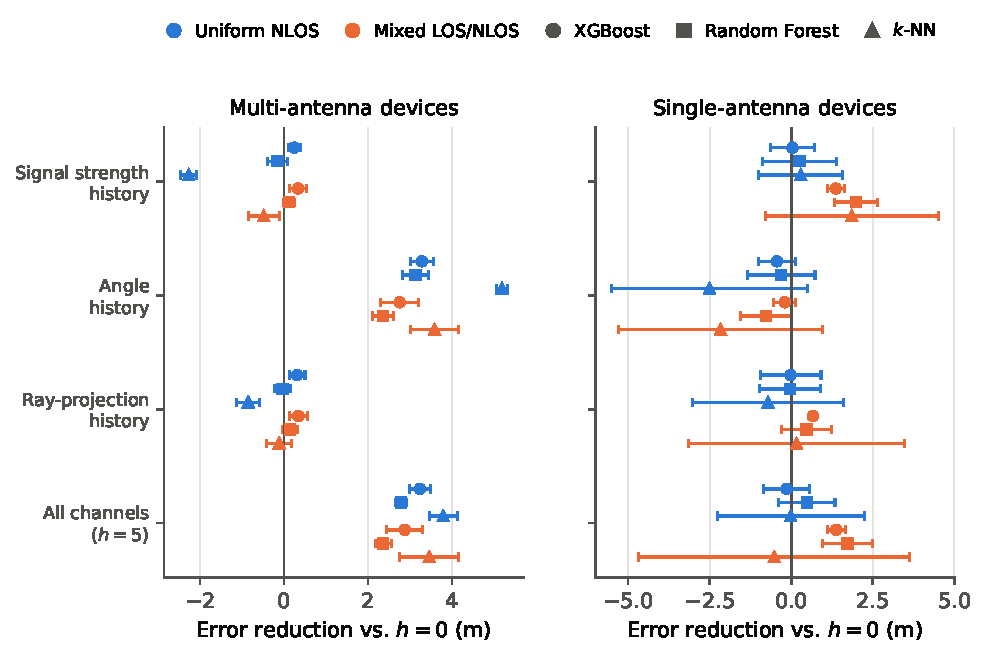
\includegraphics[width=0.95\textwidth]{fig_mechanism_conditions}
  \caption{Reduction in mean error against the $h=0$ input when history is given to one channel group at a time, or to all channels, per device group, model and dataset. Seed-paired means over five user splits with $95\%$ confidence intervals.}
  \label{fig:mechanism-conditions}
\end{figure}
% src: figure_scripts/make_figures_diagnostic.py mechanism_conditions()

% src: summary.<model>.angle_hist / rss_hist / ray_hist / full .multi.gain_vs_snap (uniform: XGB 3.28+-0.27 / 0.25+-0.14 / 0.31+-0.19 / 3.24+-0.26; RF 3.14+-0.30 / -0.15+-0.23 / -0.04+-0.18 / 2.79+-0.13; kNN 5.19+-0.12 / -2.27+-0.19 / -0.85+-0.27 / 3.79+-0.33; mixed angle: XGB 2.76+-0.45, RF 2.36+-0.25, kNN 3.59+-0.57)
The first prediction holds without exception~(Figure~\ref{fig:mechanism-conditions}). For multi-antenna devices on the uniform-NLOS data, angle history alone lowered error by $3.28 \pm 0.27\,\text{m}$ for XGBoost and $3.14 \pm 0.30\,\text{m}$ for Random Forest, as much as history on every channel~($3.24$ and $2.79\,\text{m}$). RSS history alone gave $0.25 \pm 0.14\,\text{m}$ for XGBoost and nothing detectable for Random Forest, and ray history behaved the same way. For $k$-NN, angle history alone outperformed the full window~($5.19$ against $3.79\,\text{m}$), and RSS history made it worse by $2.27\,\text{m}$, consistent with uninformative lags adding noise to its distance metric. The mixed-propagation data repeat the pattern, with angle-only gains of $2.4$ to $3.6\,\text{m}$ across the three models.

% src: per_seed.xgboost.{snap,full}.groups.multi radial_mean / tangential_mean (5-seed means 17.31 -> 14.12, 5.02 -> 4.60); single 20.23 -> 20.13, 25.22 -> 25.29
What the angle history improves is mainly the estimate of distance~(Figure~\ref{fig:radial-tangential}). For multi-antenna devices, five steps of history lowered XGBoost's mean radial error from $17.3$ to $14.1\,\text{m}$ and its tangential error only from $5.0$ to $4.6\,\text{m}$. Bearing was already well determined by the current angle measurement; the sequence of angles adds information about range. This is what Equation~(\ref{eq:dtheta-dt}) allows: for a given sideways movement, the rate at which the bearing turns falls as $1/r$, so a window of bearings carries information about distance that a single bearing does not. Single-antenna devices show no change in either component.

\begin{figure}[h]
  \centering
  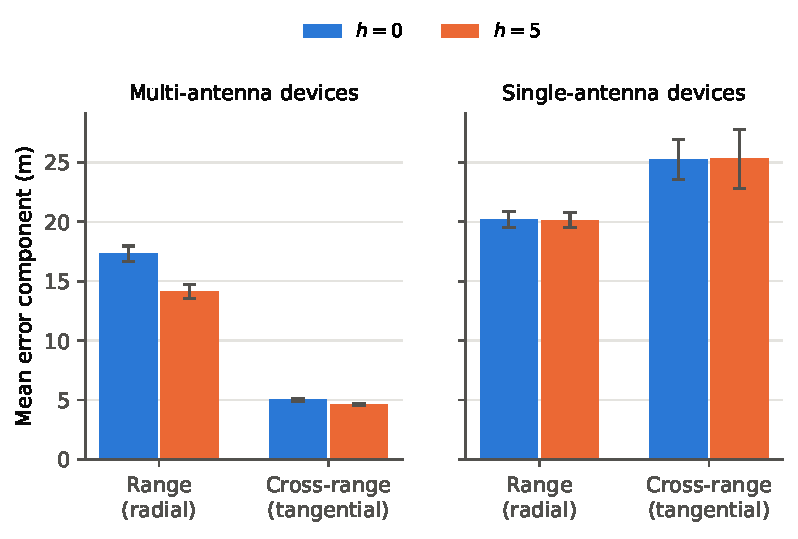
\includegraphics[width=0.75\textwidth]{fig_radial_tangential}
  \caption{Mean radial~(range) and tangential~(cross-range) components of the position error without history~($h=0$) and with five steps~($h=5$), per device group, XGBoost, macro-cell study. Means over five seeds; bars are $95\%$ confidence intervals.}
  \label{fig:radial-tangential}
\end{figure}
% src: figure_scripts/make_figures_diagnostic.py radial_tangential()

% src: summary.<model>.pure_snap.multi.gain_vs_snap (uniform: XGB -0.49+-0.14, RF -0.40+-0.21, kNN -0.33+-0.54)
The test also measures how much history the $h=0$ input already contains. Removing the first differences from the $h=0$ input raised multi-antenna error by $0.49 \pm 0.14\,\text{m}$ for XGBoost and $0.40 \pm 0.21\,\text{m}$ for Random Forest. The history gains reported in Section~\ref{sec:results-multi} are therefore measured against a baseline that already holds one step of change, and they understate the full effect of history by roughly $15\%$.

% src: summary.<model>.<cond>.single.gain_vs_snap (uniform: all CIs include zero, e.g. XGB full -0.14+-0.70; mixed: XGB rss_hist 1.36+-0.26, full 1.38+-0.27; RF rss_hist 1.99+-0.66, full 1.73+-0.77; per-seed XGB rss_hist 1.27/1.29/1.10/1.28/1.87); mixed_propagation_2026_09/seed_repeats_all_models_summary.json (single h0->h5 paired: XGB 1.66+-0.50, RF 1.55+-0.73, 1D-CNN -1.00+-0.71)
The second prediction holds on the uniform-NLOS data and fails on the mixed-propagation data. Under uniform NLOS, no channel group lowered single-antenna error for any model; every confidence interval includes zero. With mixed propagation, RSS history lowered single-antenna error for both tree ensembles, by $1.36 \pm 0.26\,\text{m}$ for XGBoost and $1.99 \pm 0.66\,\text{m}$ for Random Forest, and the gain was positive in every one of the five splits. The separate five-seed comparison of all seven models on the mixed data confirms this for the two tree ensembles, but the neural models do not share it, and the 1D-CNN's single-antenna error rises slightly with history. Section~\ref{sec:results-propagation} examines where this gain arises.

\begin{figure}[h]
  \centering
  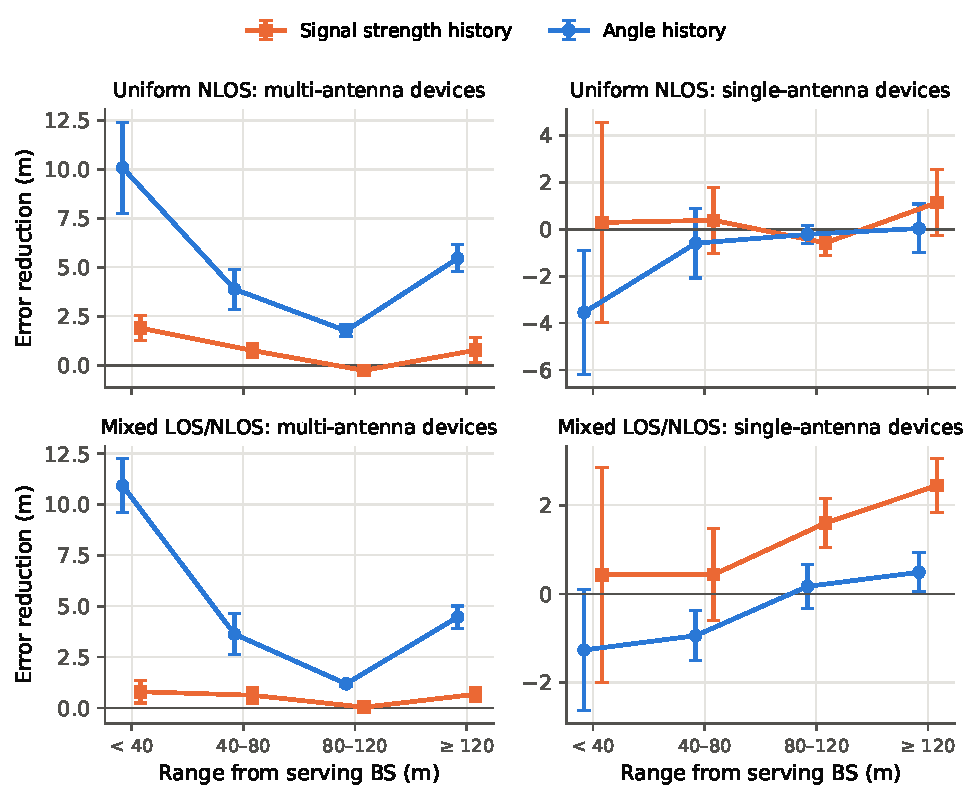
\includegraphics[width=0.85\textwidth]{fig_mechanism_by_range}
  \caption{Reduction in mean error against the $h=0$ input by range from the serving BS, for RSS-only and angle-only history, per device group and dataset, XGBoost. Seed-paired means over five user splits with $95\%$ confidence intervals. The nearest band holds about $160$ single-antenna test samples per split.}
  \label{fig:mechanism-by-range}
\end{figure}
% src: figure_scripts/make_figures_diagnostic.py mechanism_by_range(); summary.xgboost.{rss_hist,angle_hist}.*.gain_vs_snap_by_range

% src: summary.xgboost.rss_hist.multi.gain_vs_snap_by_range (uniform: <40 1.90, 40-80 0.75, 80-120 -0.26, >=120 0.77); summary.random_forest.rss_hist.multi (uniform: -0.87, 0.53, -0.39, -0.26); summary.xgboost.rss_hist.single (mixed: 0.43, 0.44, 1.60, 2.44); summary.xgboost.angle_hist.multi (uniform: 10.09, 3.89, 1.76, 5.46)
The third prediction is not supported~(Figure~\ref{fig:mechanism-by-range}). If RSS history were limited by the shrinking gradient of Equation~(\ref{eq:rss-gradient}), its gain should be largest near the BS and fall with range. For multi-antenna devices on the uniform-NLOS data, XGBoost's RSS-only gain does fall from $1.9\,\text{m}$ within $40\,\text{m}$ to slightly below zero at $80$ to $120\,\text{m}$, but it rises again beyond $120\,\text{m}$, and Random Forest shows no trend at all. For single-antenna devices on the uniform-NLOS data, too few samples lie near the BS to decide. On the mixed-propagation data, the single-antenna RSS-only gain runs the opposite way, rising from $0.4\,\text{m}$ near the BS to $2.4\,\text{m}$ beyond $120\,\text{m}$. The range-dependent account of Section~\ref{subsec:hypothesis} therefore does not explain when RSS history helps. Its other half, that the macro-cell gain depends on the angle channels, is the part the test confirms.

The angle-only gain is itself strongly range-dependent. For multi-antenna devices it falls from about $10\,\text{m}$ within $40\,\text{m}$ of the BS to under $2\,\text{m}$ at $80$ to $120\,\text{m}$, as expected if the bearing turns more slowly with distance, and then rises again to $5.5\,\text{m}$ beyond $120\,\text{m}$, where the baseline error is also largest. The rise in the farthest band is not explained by the account above.

\section{Results: Propagation and Blockage}
\label{sec:results-propagation}

\subsection{Mixed LOS and NLOS Propagation}
\label{subsec:mixed}

% src: mixed_propagation_2026_09/seed_repeats_all_models_summary.json (verdict: overall paired gains 11.4-15.4%, all significant; per-run multi/single maes for paired per-group gains; ranking h=5 16.98-17.34 for ranks 1-6); history_gain_by_zone_summary.json (h=0 test samples LOS 21,866 / NLOS 7,938)
Giving the four regions of the macro cell their own LOS or NLOS propagation leaves the main result intact~(Figure~\ref{fig:mixed-gain}). About three quarters of test samples now fall in LOS regions. History lowered the overall error of all seven models, by $11$ to $15\%$, with every seed-paired confidence interval clear of zero. For multi-antenna devices the gains are $2.3$ to $3.9\,\text{m}$, as on the uniform-NLOS data, and the six trained models other than $k$-NN again lie within $0.4\,\text{m}$ of each other. The single-antenna result differs: both tree ensembles now gain about $1.6\,\text{m}$ for single-antenna devices, while the neural models and $k$-NN do not.

\begin{figure}[h]
  \centering
  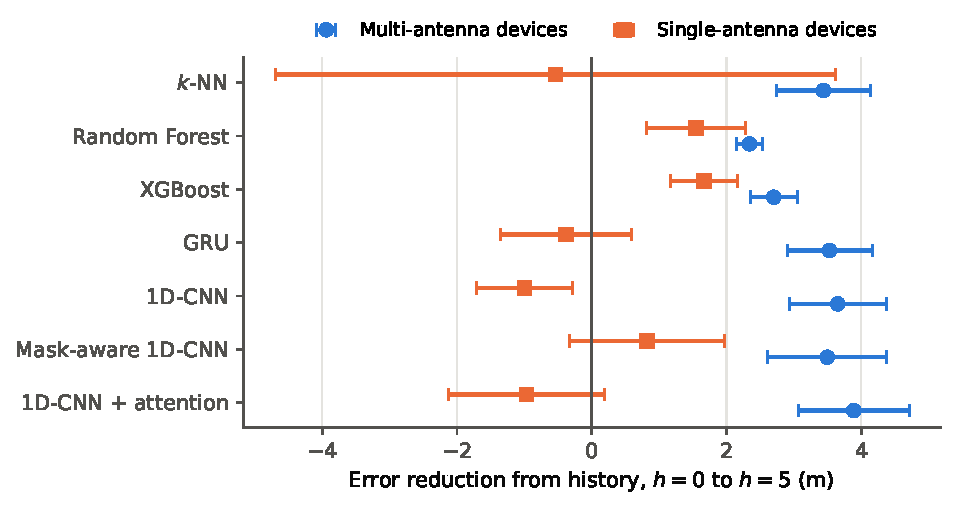
\includegraphics[width=0.8\textwidth]{fig_mixed_history_gain_ci}
  \caption{Reduction in mean error from adding history~($h=0$ to $h=5$), per model and device group, mixed-propagation realization of the macro-cell study. Seed-paired means over five user splits with $95\%$ confidence intervals.}
  \label{fig:mixed-gain}
\end{figure}
% src: figure_scripts/make_figures_diagnostic.py mixed_history_gain_ci()

% src: mixed_propagation_2026_09/pathloss_fit_summary.json zones.LOS (gamma 2.578, sigma 7.67 dB, R^2 0.261) and zones.NLOS (gamma 3.595, sigma 11.89 dB, R^2 0.069); per-region fits are unstable (e.g. residential gamma 6.92) and are not used; note: the fit assigns regions geometrically from the Voronoi centres
Signal strength is more informative about range in the LOS regions. A path-loss fit to the LOS samples gives $\gamma = 2.58$ with a shadowing spread of $7.7\,\text{dB}$, and range explains $26\%$ of the variance in RSS. In the NLOS regions the fit gives $\gamma = 3.60$, a spread of $11.9\,\text{dB}$, and only $7\%$ of the variance explained.

% src: mixed_propagation_2026_09/history_gain_by_zone_summary.json verdict (LOS 15.94%, NLOS 8.65%; mean range LOS 90.1 m, NLOS 96.8 m; XGBoost, seed 42); diagnostics_2026_10/mixed_propagation summary.<model>.<cond>.multi.gain_vs_snap_by_los (XGB angle LOS 3.12+-0.62, NLOS 1.51+-0.16; RF angle 2.68+-0.33 / 1.25+-0.15; XGB rss 0.33+-0.22 / 0.38+-0.25)
History helps more in LOS regions, and the difference lies in the angle channels~(Figure~\ref{fig:los-nlos}). In a single XGBoost run, history lowered error by $15.9\%$ in LOS regions and by $8.7\%$ in NLOS regions. Mean range is slightly shorter in the LOS regions~($90$ against $97\,\text{m}$), but too little to account for the difference. Splitting the channel-group test by region shows where the difference comes from: for multi-antenna devices, angle history lowered XGBoost's error by $3.12 \pm 0.62\,\text{m}$ in LOS regions and by $1.51 \pm 0.16\,\text{m}$ in NLOS regions, and Random Forest shows the same ratio, while RSS history gave the same small gain in both. Under LOS a single dominant path makes the measured angle a steadier function of position, which is consistent with a sequence of angles carrying more about range there.

\begin{figure}[h]
  \centering
  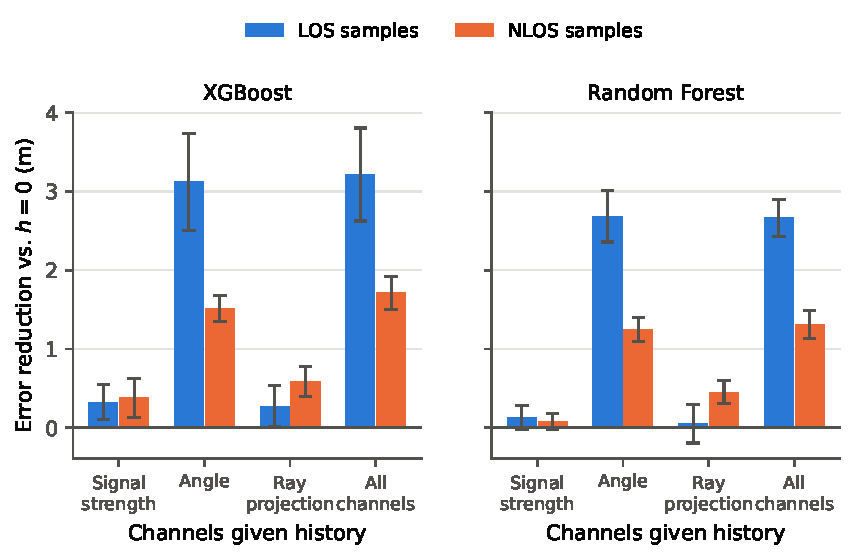
\includegraphics[width=0.85\textwidth]{fig_los_nlos_channels}
  \caption{Reduction in mean error against the $h=0$ input for multi-antenna devices, by channel group given history and by whether the current sample lies in a LOS or NLOS region, mixed-propagation realization. Seed-paired means over five user splits with $95\%$ confidence intervals.}
  \label{fig:los-nlos}
\end{figure}
% src: figure_scripts/make_figures_diagnostic.py los_nlos_channels()

% src: diagnostics_2026_10/mixed_propagation summary.xgboost.rss_hist.single.gain_vs_snap_by_los (LOS 1.28+-0.42, NLOS 1.53+-0.87); exploratory check on errors_first_seed.npz (seed 42, full vs snap, single-antenna samples whose six-step window contains both LOS and NLOS samples, 15% of single-antenna samples): RF 2.85 vs 1.06 m, kNN 2.92 vs 0.84 m, XGB 1.40 vs 1.16 m (scratch analysis analyze_b6_npz.py)
The single-antenna gain from RSS history on these data is not explained by the cleaner LOS path-loss relation: XGBoost's RSS-only gain is $1.28 \pm 0.42\,\text{m}$ for samples in LOS regions and $1.53 \pm 0.87\,\text{m}$ for samples in NLOS regions. A possible source is the step in signal strength that occurs when a device crosses from one propagation region to another, which marks a location the window can recognize. In one split, the gain for Random Forest and $k$-NN was about three times larger when the history window spanned such a crossing than when it did not~($2.9$ against $1.1\,\text{m}$ for Random Forest), but XGBoost showed no such difference, and windows without a crossing still gained about $1\,\text{m}$. This is a lead from a single split with ten single-antenna users, not an explanation, and the single-antenna gain on mixed-propagation data remains open.

\subsection{A Blocked Line of Sight}
\label{subsec:blocked}

% src: CONTINUE_HERE.md §4 (prediction: advantage grows with blockage duration until the pre-blockage heading stops being informative, then decays); blocked_los_2026_09/b6_seed*_summary.json (5 seeds, XGBoost, h in {0,5}): blocked gain 28.9/28.5/36.5/28.6/22.8% mean 29.1 sd 4.9; unblocked mean 22.5 sd 6.0; blocked h0 18.90 -> h5 13.45 m, unblocked 25.08 -> 19.59 m; paired blocked-minus-unblocked gain in metres -0.04 +- 0.46; by width 24.1/25.4/23.8/26.8/31.6/27.4/26.3/32.2% with mean n ~59/90/175/386/899/1039/1544/1536
The blocked line-of-sight scenario was designed to test whether history becomes more valuable as a blockage lengthens, up to the point where the heading observed before the blockage stops being informative, after which its value should decay. Over five seeds, with XGBoost at $h=0$ and $h=5$, history lowered the error inside the blocked stretch by $29\%$ on average and outside it by $22.5\%$. In meters the two reductions are the same, about $5.5\,\text{m}$, because the error without history is lower inside the blocked stretch~($18.9\,\text{m}$) than outside it~($25.1\,\text{m}$). The reduction does not rise and fall with the width of the blocked strip~(Figure~\ref{fig:blocked}): it stays between $24$ and $32\%$ from $5$ to $150\,\text{m}$, and the narrowest strips, with fewer than $200$ samples each, vary widely from seed to seed. History therefore keeps its value through a blockage of any length tested, but the predicted dependence on blockage length does not appear.

\begin{figure}[h]
  \centering
  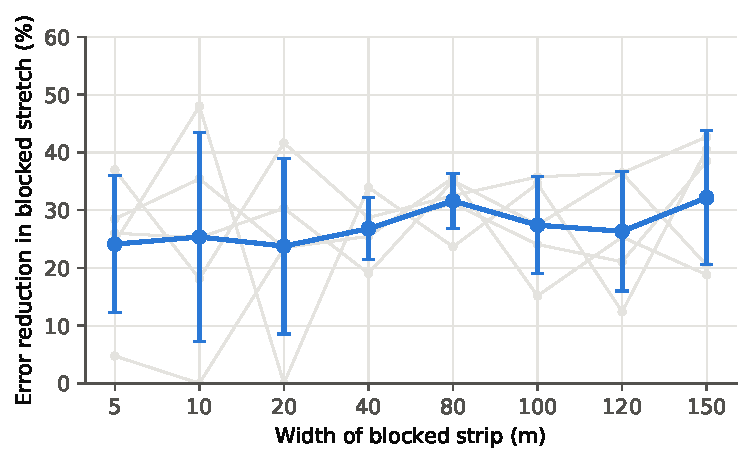
\includegraphics[width=0.7\textwidth]{fig_blocked_by_width}
  \caption{Reduction in mean error from adding history~($h=0$ to $h=5$) inside the blocked stretch, by width of the blocked strip, XGBoost. Gray lines are the five individual seeds; the blue line is their mean with $\pm1$ standard deviation.}
  \label{fig:blocked}
\end{figure}
% src: figure_scripts/make_figures_diagnostic.py blocked_by_width()

\section{Discussion}
\label{sec:discussion}

\pending{[Awaiting Gilad's results: drafted once the mechanism experiment is in. It covers why the gain from history depends on device hardware and range, how the controlled grid and the macro cell differ as regimes, the single-user regression runs in which history did not help, what the evidence does not support, and the practical case for a small boosted-tree model.]}
             % placeholder: drafted after the mechanism diagnostic
\section{Limitations}
\label{sec:limitations}

% src: FINAL_REPORT.md §9 items 1, 2, 3, 4, 5; §10 item 6 (device groups imposed at feature level); model_zoo.py train_deep (test-based stopping); technical_documentation.md §7.2.1 vs §7.2.6 (single-run variability)
All results come from simulation. Spatial consistency, the property that gives a measurement sequence its information, is a feature of the channel model here; real channels exhibit it, but also add non-stationarity, hardware impairments and calibration drift that the simulations omit. The trajectories are likewise synthetic: they are generated on a grid graph rather than drawn from measured traces, and lack the road geometry and stop-and-go behavior of real movement.

The two device groups of the macro-cell study share one simulated channel, since every UE is simulated with the same omnidirectional array and the absence of an angle is imposed when features are built. The contrast between the groups is therefore a contrast in available measurements rather than in physical hardware. The $85/15$ population mix is an assumption, which is why every result is reported per group rather than for the blend. Each test split of $47$ users contains only $5$ to $10$ single-antenna devices, so their errors carry much wider seed-to-seed uncertainty than those of multi-antenna devices, and any result resting on the nearest range band rests on a few hundred single-antenna samples at most.
% src: diagnostics_2026_10 user_counts (10, 7, 6, 10, 5)

% src: diagnostics_2026_10 meta.models (xgboost, random_forest, knn); mixed_propagation_2026_09/seed_repeats_all_models_summary.json (neural single-antenna gains not significant or negative)
The channel-group test of Section~\ref{sec:results-mechanism} covers $k$-NN, Random Forest and XGBoost only, so the finding that the angle channels carry the gain is established for these three models and inferred for the neural ones. The single-antenna gain that the tree ensembles obtain from RSS history under mixed propagation is unexplained, and the region-crossing account of Section~\ref{subsec:mixed} rests on a single split.

Because every step of a walk advances exactly one grid cell, history depth measures both the number of samples and the distance travelled, and the two cannot be separated in these data; doing so requires simulations with variable step length or variable sampling rate. The neural models chose their stopping epoch on the test users, which flatters their absolute errors and any comparison with the tree and instance-based models, though not the comparisons between depths of one model. Finally, the controlled-grid results are single runs, and repeated runs of the same configuration differ by two to three percentage points, so only their larger effects are interpreted.

\section{Conclusion}
\label{sec:conclusion}

\pending{[Awaiting Gilad's results: drafted once the mechanism experiment is in, with the follow-up work it points to.]}
             % placeholder: drafted after the mechanism diagnostic

\nocite{*}
\bibliographystyle{IEEEtran}
\bibliography{reference}

\appendices
\renewcommand{\thesubsection}{\thesection-\arabic{subsection}}
\renewcommand{\thesubsectiondis}{\thesection-\arabic{subsection}}
\newpage \section{Code and Data Availability}
\label{app:reproducibility}

% src: FINAL_REPORT.md Appendix A; results_of_record/MANIFEST.md
The simulation configurations, generation scripts, feature pipeline, model definitions and analysis scripts are available in the project repository~(\url{https://github.com/slash827/CSI-Location}). Simulated datasets are regenerated from the configurations rather than distributed. Every number in this report is drawn from machine-written summary files kept in the repository alongside an index of the experiment that produced each one. The global random seed is $42$; the five-seed repeats use seeds $42$, $1$, $7$, $13$ and $99$.

\newpage \section{Model Hyperparameters}
\label{app:hyperparameters}

% src: CSI-Location experiments_ablation/model_zoo.py (build_classical, protocol constants, architectures); master_benchmark_rerun_summary.json (n_params)
\begin{table}[h]
  \centering
  \caption{Macro-cell model configurations. Hyperparameters are identical at every history depth.}
  \label{tab:hyperparameters}
  \small
  \begin{tabularx}{\textwidth}{@{}lX@{}}
    \toprule
    Model & Configuration \\
    \midrule
    $k$-NN & $k=5$ neighbors, Euclidean distance on standardized features \\
    Random Forest & $150$ trees, maximum depth $16$, minimum leaf size $5$, $\sqrt{d}$ features per split \\
    XGBoost & $50$ trees, maximum depth $5$, learning rate $0.15$, row and column subsampling $0.8$, one output per tree \\
    1D-CNN & Three convolutional layers~($32$, $64$, $128$ filters, kernel $3$) with batch normalization and dropout $0.35$, global average pooling, a shared $128$-unit trunk with the static device features, and position, speed and uncertainty heads; $66{,}500$ parameters \\
    Mask-aware 1D-CNN & As the 1D-CNN, with an additional AoA-validity input channel; $66{,}596$ parameters \\
    1D-CNN + attention & As the 1D-CNN, followed by a four-head temporal self-attention block with learned positional embeddings; $199{,}748$ parameters \\
    GRU & Two recurrent layers of $128$ units, dropout $0.30$, a $256$-unit shared trunk and the same three heads; $254{,}468$ parameters \\
    Neural training & AdamW, learning rate $3\times10^{-4}$, weight decay $10^{-2}$, batch size $512$, Huber loss with weights $1.0$, $0.2$ and $0.05$ on position, speed and uncertainty, at most $60$ epochs, early stopping with patience $8$ \\
    \bottomrule
  \end{tabularx}
\end{table}

\newpage \section{Supplementary Results}
\label{app:supplementary}

\begin{table}[h]
  \centering
  \caption{Effect of history~($h=0$ to $h=5$) per model and device group, macro-cell study. Errors are means over five seeds; gains are seed-paired, with $95\%$ confidence intervals. Training time and time to predict $1000$ positions come from a single run.}
  \label{tab:history-gain}
  \small
  \begin{tabular}{@{}lrrrrrr@{}}
    \toprule
     & \multicolumn{2}{c}{Multi-antenna devices} & \multicolumn{2}{c}{Single-antenna devices} & \multicolumn{2}{c}{Cost} \\
    \cmidrule(lr){2-3}\cmidrule(lr){4-5}\cmidrule(l){6-7}
    Model & Error, $h=0$ & Gain & Error, $h=0$ & Gain & Training & ms per 1000 \\
    \midrule
    $k$-NN & $23.4\,\text{m}$ & $3.77 \pm 0.33\,\text{m}$ & $46.2\,\text{m}$ & $-0.11 \pm 2.32\,\text{m}$ & $1\,\text{s}$ & $577$ \\
    Random Forest & $18.8\,\text{m}$ & $2.75 \pm 0.13\,\text{m}$ & $36.6\,\text{m}$ & $0.32 \pm 0.86\,\text{m}$ & $34\,\text{s}$ & $102$ \\
    XGBoost & $18.8\,\text{m}$ & $3.16 \pm 0.34\,\text{m}$ & $35.8\,\text{m}$ & $0.06 \pm 0.18\,\text{m}$ & $4\,\text{s}$ & $1.7$ \\
    GRU & $19.3\,\text{m}$ & $3.54 \pm 0.66\,\text{m}$ & $36.7\,\text{m}$ & $-0.26 \pm 0.76\,\text{m}$ & $166\,\text{s}$ & $31$ \\
    1D-CNN & $19.5\,\text{m}$ & $3.73 \pm 0.85\,\text{m}$ & $36.0\,\text{m}$ & $-1.16 \pm 1.82\,\text{m}$ & $197\,\text{s}$ & $14$ \\
    Mask-aware 1D-CNN & $19.3\,\text{m}$ & $3.47 \pm 0.75\,\text{m}$ & $34.8\,\text{m}$ & $0.25 \pm 0.82\,\text{m}$ & $182\,\text{s}$ & $18$ \\
    1D-CNN + attention & $19.5\,\text{m}$ & $4.06 \pm 0.74\,\text{m}$ & $35.9\,\text{m}$ & $-1.39 \pm 3.28\,\text{m}$ & $212\,\text{s}$ & $23$ \\
    \bottomrule
  \end{tabular}
\end{table}
% src: seed_repeats_all_models_summary.json per_config runs (seed-paired per-group differences); master_benchmark_rerun_summary.json scorecard (train_time_sec, latency_ms_per_1k; k-NN cost row is the h=5 model)

\begin{table}[h]
  \centering
  \caption{Macro-cell study: overall mean error~(m) by history depth for every model, single seed. These are the values behind Figure~\ref{fig:history-by-group}, pooled over both device groups.}
  \label{tab:supp-depth}
  \small
  \begin{tabular}{@{}lrrrrr@{}}
    \toprule
    Model & $h=0$ & $h=1$ & $h=3$ & $h=5$ & $h=10$ \\
    \midrule
    $k$-NN & 27.44 & 25.43 & 24.07 & 23.98 & 24.49 \\
    Random Forest & 22.11 & 20.91 & 19.77 & 19.42 & 19.34 \\
    XGBoost & 22.35 & 21.12 & 19.80 & 19.43 & 19.03 \\
    GRU & 22.72 & 21.43 & 19.97 & 19.36 & 18.47 \\
    1D-CNN & 22.85 & 20.62 & 19.52 & 19.27 & 19.15 \\
    Mask-aware 1D-CNN & 22.10 & 20.26 & 19.24 & 18.75 & 18.26 \\
    1D-CNN + attention & 22.54 & 21.02 & 19.40 & 18.90 & 18.19 \\
    \bottomrule
  \end{tabular}
\end{table}
% src: history_sweep_all_models_summary.json curves.*.h*.mae (seed 42)

\begin{table}[h]
  \centering
  \caption{Macro-cell study: overall mean error~(m) over five seeds, with $95\%$ confidence interval and full range across seeds, and the seed-paired overall gain from $h=0$ to $h=5$.}
  \label{tab:supp-seeds}
  \small
  \begin{tabular}{@{}lrrrrr@{}}
    \toprule
    Model & $h=0$ & Spread, $h=0$ & $h=5$ & Spread, $h=5$ & Paired gain \\
    \midrule
    $k$-NN & $27.07 \pm 0.64$ & 1.85 & $23.86 \pm 0.85$ & 2.53 & $3.22 \pm 0.27$ \\
    Random Forest & $21.66 \pm 0.46$ & 1.24 & $19.28 \pm 0.39$ & 1.19 & $2.38 \pm 0.20$ \\
    XGBoost & $21.51 \pm 0.50$ & 1.35 & $18.87 \pm 0.46$ & 1.12 & $2.65 \pm 0.29$ \\
    GRU & $22.03 \pm 0.56$ & 1.27 & $19.09 \pm 0.49$ & 1.36 & $2.95 \pm 0.49$ \\
    1D-CNN & $22.10 \pm 0.62$ & 1.46 & $19.12 \pm 0.52$ & 1.31 & $2.98 \pm 0.63$ \\
    Mask-aware 1D-CNN & $21.74 \pm 0.59$ & 1.56 & $18.81 \pm 0.52$ & 1.46 & $2.93 \pm 0.58$ \\
    1D-CNN + attention & $22.08 \pm 0.61$ & 1.61 & $18.84 \pm 0.44$ & 1.30 & $3.24 \pm 0.63$ \\
    \bottomrule
  \end{tabular}
\end{table}
% src: seed_repeats_all_models_summary.json per_config (mae_mean, mae_ci95, mae_spread) and verdict (gain_mean_m, gain_ci95_m)

\begin{table}[h]
  \centering
  \caption{Macro-cell study: overall mean error~(m) with fixed hyperparameters and with hyperparameters re-tuned separately at each depth on training users only, single seed.}
  \label{tab:supp-retune}
  \small
  \begin{tabular}{@{}lrrrr@{}}
    \toprule
     & \multicolumn{2}{c}{XGBoost} & \multicolumn{2}{c}{Random Forest} \\
    \cmidrule(lr){2-3}\cmidrule(l){4-5}
    Depth & Fixed & Re-tuned & Fixed & Re-tuned \\
    \midrule
    $h=0$ & 22.35 & 21.91 & 22.11 & 22.05 \\
    $h=1$ & 21.12 & 21.20 & 20.91 & 20.84 \\
    $h=3$ & 19.80 & 19.66 & 19.77 & 19.81 \\
    $h=5$ & 19.43 & 19.07 & 19.42 & 19.40 \\
    $h=10$ & 19.03 & 18.97 & 19.34 & 19.30 \\
    \bottomrule
  \end{tabular}
\end{table}
% src: xgb_per_h_retune_summary.json, rf_per_h_retune_summary.json (as transcribed in FINAL_REPORT.md §5.5)


\end{document}
